%%%%%%%%%%%%%%%%%%%%%%%%%%%%%%%%%%%%%%%%%%%%%%%%%%%%%%%%%%%%%%%%%%%%%%%%%%%%%%%%%%%%%%%%%
% This is a LaTeX template for Bachelor or Master theses at ZHAW, in accordance with the
% guidelines provided here:
% https://www.zhaw.ch/en/lsfm/study/studiweb/master-ls/masters-thesis/
%
%
% This template is based on previous works by:
% Steve Gunn (http://users.ecs.soton.ac.uk/srg/softwaretools/document/templates/)
% Sunil Patel (http://www.sunilpatel.co.uk/thesis-template/)
% Matteo Delucchi (https://github.com/matteodelucchi/ZHAW_thesis-template)
%
% University specific changes were made by:
% Matteo Delucchi
% Norman Juchler
%
% Template license:
% CC BY-NC-SA 3.0 (http://creativecommons.org/licenses/by-nc-sa/3.0/)
%%%%%%%%%%%%%%%%%%%%%%%%%%%%%%%%%%%%%%%%%%%%%%%%%%%%%%%%%%%%%%%%%%%%%%%%%%%%%%%%%%%%%%%%%

%----------------------------------------------------------------------------------------
% DOCUMENT SPECIFICATION
%----------------------------------------------------------------------------------------
\documentclass[
    11pt,                      % Default font size
    %oneside,                  % One-side binding. Default: Two-side binding / alternating margins
    english,                   % Language. Use ngerman for German (Neue Rechtschreibung)
    singlespacing,             % Spacing option: singlespacing, onehalfspacing or doublespacing
    %nolistspacing,            % Set spacing in lists to single
    %draft,                    % Enable draft mode: no pictures, no links, overfull hboxes indicated
    liststotoc,               % Include list of figures/tables/etc in the table of contents
    %toctotoc,                 % Include the main table of contents to the table of contents
    parskip,                  % Add vertical space between paragraphs
    %nohyperref,               % Disable links in the entire document
    headsepline,               % Show a horizontal line under the header
    %chapterinoneline,         % Place the chapter title and chapter number on one line
    consistentlayout,          % Have the same layout for special chapters:
                               % declaration, abstract and acknowledgements
]{MastersDoctoralThesis}

% Uncomment the following lines to only include a subset of chapters.
% This is useful for long documents, as typesetting takes a bit of time
%\includeonly{
%    Front/titlepage,
%    Front/imprint,
%    Front/abstract,
%    %Front/declaration,
%    %Front/acknowledgements,
%    %Front/symbols,
%    Chapters/Chapter1,
%    %Chapters/Chapter2
%    }


%----------------------------------------------------------------------------------------
% PREAMBLE: PACKAGES AND CONFIGURATIONS
%----------------------------------------------------------------------------------------
% !TEX root = main.tex

%----------------------------
%   Fonts and characters
%----------------------------

% Support for special characters
\usepackage[utf8]{inputenc}    % Specify input encoding
\usepackage[T1]{fontenc}       % Specify font encoding

% Set main fonts
% Fonts catalogue: https://tug.org/FontCatalogue/
\usepackage{mathpazo}          % Use the Palatino font by default
\usepackage{beramono}          % Override the monospace/typewriter font

% ZHAW title font
% Try to load Helvetica Rounded Bold, and OpenType font.
% Loading OTF or system fonts is possible with XeLaTeX.
% If the document is compiled using pdfLaTeX, resort 
\usepackage{ifxetex}
\ifxetex
    \usepackage{fontspec}
    \newfontfamily\zhawtitlefont{Helvetica Rounded Bold}
\else
    \newcommand{\zhawtitlefont}{\scshape}
\fi

%\usepackage[scaled]{helvet}

%----------------------------
%   Environments
%----------------------------

\usepackage{caption}           % Customized caption
\usepackage{subcaption}        % Subfigure captions
\usepackage{makecell}          % Per-cell formatting in tables (\makecell)
\usepackage{pdfpages}          % Required to include PDF files/graphics (\includepdf)

\usepackage{todonotes}         % Introduces the command \todo
\setlength{\marginparwidth}{2.5cm} % Adjust this if the todo notes are out of margins

% Create boxes as follows:
% \begin{colorbox}{red}{2}
\usepackage{tcolorbox}
\newtcolorbox{textbox}[2]{
    arc=3pt,
    boxrule=#2pt,
    colback=#1!25!white,
    width=\textwidth,
    halign=left,
    valign=center,
    colframe=#1!75!black
}

%----------------------------
%   Colors
%----------------------------

% Set up colors
\usepackage{xcolor}
% ZHAW Blue: Pantone 2945 U / R0 G100 B166
\definecolor{zhawblue}{rgb}{0.00, 0.39, 0.65}
% Colors related to code listings
\definecolor{codegreen}{rgb}{0,0.6,0}
\definecolor{codegray}{rgb}{0.5,0.5,0.5}
\definecolor{codepurple}{rgb}{0.58,0,0.82}
\definecolor{codebackground}{rgb}{0.93,0.94,0.95}

%----------------------------
%   Code listings
%----------------------------

% Setup code listings
\usepackage{listings}
\lstdefinestyle{mystyle}{
    backgroundcolor=\color{codebackground},   
    commentstyle=\color{codegreen},
    keywordstyle=\color{magenta},
    numberstyle=\tiny\color{codegray},
    stringstyle=\color{codepurple},
    basicstyle=\ttfamily\footnotesize,
    breakatwhitespace=false,
    breaklines=true,
%    captionpos=b,
    keepspaces=true,
    numbers=left,
    numbersep=5pt,
    showspaces=false,
    showstringspaces=false,
    showtabs=false,
    tabsize=4
}
\lstset{style=mystyle}

% minted is an alternative code listing package. (See chapter 2)
% For it to run successfully, ensure the following:
% - the Python package Pygments. Install with the following command:
%       python -m pip install Pygments
% - pdflatex (or xelatex) is executed with the flag --shell-escape
%   If you are using a TEX editor, you can modify the typesetting 
%   command somewhere in the settings.
%\usepackage[outputdir=build]{minted}
%\usemintedstyle{xcode}
% For fancier coloring schemes, see here:
% https://tex.stackexchange.com/questions/585582
% One could also create an own style in Pygments
% https://pygments.org/docs/styles/#creating-own-styles

%----------------------------
%   References
%----------------------------

% Set up references
\usepackage[
    backref=true,
    backend=biber,             % Use biber backend (an external tool)
    sorting=none,              % Enumerates the reference in order of their appearance
    hyperref=true,
    mincitenames=1,
    maxcitenames=1,
    uniquelist=false,
    eprint=false,doi=false,isbn=false,url=false, % https://tex.stackexchange.com/a/23118
    % style=numeric-comp         % Choose here your preferred citation style
    % style=authoryear-comp        % breaks repeated cites
    style=authoryear        % Choose here your preferred citation style
]{biblatex}

% \addbibresource{example.bib}   % The filename of the bibliography
\addbibresource{manual_all.bib}


%%%%%%%%%%%%%%%%%%%%%%%%%%%%%%%%%%%%%%%%%%%%%%%%%%%%%%
% backref for cited on pages...
% https://tex.stackexchange.com/a/36308
\DefineBibliographyStrings{english}{%
  backrefpage  = {cited on page}, % originally "cited on page"
  backrefpages = {cited on pages},% originally "cited on pages"
}

%%%%%%%%%%%%%%%%%%%%%%%%%%%%%%%%%%%%%%%%%%%%%%%%%%%%%%
% linebreak before backref
% https://tex.stackexchange.com/a/76136
\setlength\bibitemsep{1.7\itemsep}
\renewcommand*{\finentrypunct}{}
\renewbibmacro*{pageref}{%
  \addperiod% NEW
  \iflistundef{pageref} {}
    {
    \begin{flushright}
    % \linebreak
    \footnotesize\printtext[parens]{% NEW
       \ifnumgreater{\value{pageref}}{1}
         {\bibstring{backrefpages}\ppspace}
     {\bibstring{backrefpage}\ppspace}%
       \printlist[pageref][-\value{listtotal}]{pageref}}
    \end{flushright}
    }}% NEW
%%%%%%%%%%%%%%%%%%%%%%%%%%%%%%%%%%%%%%%%%%%%%%%%%%%%%%

%%%%%%%%%%%%%%%%%%%%%%%%%%%%%%%%%%%%%%%%%%%%%%%%%%%%%%
% https://tex.stackexchange.com/questions/1687/hyperlink-name-with-biblatex-authoryear
%%%%%%%%%%%%%%%%%%%%%%%%%
% duplicated works but no hyper
% \makeatletter
% \newrobustcmd*{\parentexttrack}[1]{%
%   \begingroup
%   \blx@blxinit
%   \blx@setsfcodes
%   \blx@bibopenparen#1\blx@bibcloseparen
%   \endgroup}
% \AtEveryCite{%
%   \let\parentext=\parentexttrack%
%   \let\bibopenparen=\bibopenbracket%
%   \let\bibcloseparen=\bibclosebracket}
% \makeatother
%%%%%%%%%%%%%%%%%%%%%%%%%

%%%%%%%%%%%%%%%%%%%%%%%%%
% duplicated NOT work (with authoryear-comp) but hyper yes
\DeclareCiteCommand{\parencite}
  {\usebibmacro{prenote}}
  {\usebibmacro{citeindex}%
   \printtext[bibhyperref]{[\usebibmacro{cite}]}}
  %                        ^                  ^
  {\multicitedelim}
  {\usebibmacro{postnote}}
% \makeatletter
% \newrobustcmd*{\parentexttrack}[1]{%
%   \begingroup
%   \blx@blxinit
%   \blx@setsfcodes
%   \blx@bibopenparen#1\blx@bibcloseparen
%   \endgroup}

% \AtEveryCite{%
%   \let\parentext=\parentexttrack%
%   \let\bibopenparen=\bibopenbracket%
%   \let\bibcloseparen=\bibclosebracket}
% \makeatother
%%%%%%%%%%%%%%%%%%%%%%%%%
%%%%%%%%%%%%%%%%%%%%%%%%%%%%%%%%%%%%%%%%%%%%%%%%%%%%%%

% https://tex.stackexchange.com/a/318312
\usepackage{letltxmacro}\LetLtxMacro{\cite}{\parencite} % remove / comment to use numeric-comp biblatex style
\renewcommand*{\nameyeardelim}{\addcomma\space}

\usepackage[autostyle=true]{csquotes}
                               % Required to generate language-dependent quotes 
                               % in the bibliography

%----------------------------------------------------------------------------------------
%   MARGIN SETTINGS
%----------------------------------------------------------------------------------------

\geometry{
    paper=a4paper,      % Change to letterpaper for US letter
    inner=2.5cm,        % Inner margin
    outer=3.8cm,        % Outer margin
    top=1.5cm,          % Top margin
    bottom=1.5cm,       % Bottom margin
    bindingoffset=.5cm, % Binding offset
    %showframe,         % Show the type block of the page
}
\setlength{\parskip}{1em}
\usepackage{enumitem}          % Layout control for list environments (e.g, itemize)
%\setlist{noitemsep}           % Suppress extra spaces between items
%\setlist{nosep}               % Suppress spaces before/after list environments

% \pdfcompresslevel=0
% \pdfobjcompresslevel=0

\newcommand{\withbigtikz}[0]{} % uncomment to include c5 graphs
% \newcommand{\csvfilesuffix}[0]{fast}
% \newcommand{\csvfilesuffix}[0]{spline}
\newcommand{\csvfilesuffix}[0]{normal}

\usepackage{amsmath,bm} % bm redefines \boldsymbol{Symbol}!
% \usepackage{setspace} % allows spacing in arrays?


%%%%%%%%%%%%%%%%%%%%%%%%%%%%%%%%%%%%%%%%%%%%%%%%%%%%%
% shrink font size locally
% (fixes problem with caption font size in tikz sub-figures)
% https://tex.stackexchange.com/questions/250457/font-scaling-shrink-all-fontsizes-locally
\usepackage{geometry}
\makeatletter
\let\zzfontsize\fontsize
\def\zz#1#2{{%
    \def\fontsize##1##2{%
      \@defaultunits\@tempdima##1pt\relax\@nnil
      \@defaultunits\@tempdimb##1pt\relax\@nnil
      \zzfontsize{#1\@tempdima}{#1\@tempdimb}}#2}}
\makeatother
% NOTE: 0.64 is the magic number for font size footnotesize
\newcommand{\captiontikz}[2]{\zz{0.64}{\caption{#1}\label{#2}}}
% \newcommand{\captiontikz}[1]{\caption{#1}}
%%%%%%%%%%%%%%%%%%%%%%%%%%%%%%%%%%%%%%%%%%%%%%%%%%%%%
% image page with different margins
% https://tex.stackexchange.com/a/78285
\usepackage{afterpage}
%%%%%%%%%%%%%%%%%%%%%%%%%%%%%%%%%%%%%%%%%%%%%%%%%%%%%

\usepackage{tabularx}


%%%%%%%%%%%%%%%%
% table configs: https://tex.stackexchange.com/a/176780
\usepackage{makecell}
\renewcommand\theadalign{bc}
\renewcommand\theadfont{\bfseries}
\renewcommand\theadgape{\Gape[4pt]}
\renewcommand\cellgape{\Gape[4pt]}
%%%%%%%%%%%%%%%%


\usepackage{dashrule}

\usepackage{marginnote}
\usepackage{qrcode}
% \usepackage{pst-barcode}
% \usepackage{auto-pst-pdf}

\usepackage{amssymb}




%%%%%%%%%%%%%%%%%%%%%%%%%%%%%%%%%%%%%%%%%%%%%%%%%%%%%
% force right margin notes
% https://tex.stackexchange.com/a/599049
\usepackage{ifthen,changepage}
\usepackage{xargs}
\newcommandx{\leftmarginnote}[2][2=0pt]
{\checkoddpage
  \ifoddpage
    {\reversemarginpar\marginnote{#1}[#2]}
  \else
    {\marginnote{#1}[#2]}
  \fi}
\newcommandx{\rightmarginnote}[2][2=0pt]
{\checkoddpage
  \ifoddpage
    {\marginnote{#1}[#2]}
  \else
    {\reversemarginpar\marginnote{#1}[#2]}
  \fi}
%%%%%%%%%%%%%%%%%%%%%%%%%%%%%%%%%%%%%%%%%%%%%%%%%%%%%



%%%%%%%%%%%%%%%%%%%%%%%%%%%%%%%%%%%%%%%%%%%%%%%%%%%%%
% revisited equations in marginnote
% https://tex.stackexchange.com/questions/25491/manual-customizable-reference-text
% \newcommand{\futurev}[1]{\marginnote{\footnotesize (revisited~\hyperref[#1]{later})}[0cm]}
\newcommand{\revhspace}[0]{\hspace{.3cm}}
\newcommand{\futurev}[1]{{
    \scriptsize
    \rightmarginnote{\revhspace
      \hyperref[#1]{{\footnotesize revisited}~$\downarrow$}
    }[0cm]}}
\newcommand{\prevrev}[1]{{
    \scriptsize
    \rightmarginnote{\revhspace
      \hyperref[#1]{{\footnotesize revisited}~$\uparrow$}
    }[0cm]}}
\newcommand{\prevfuturev}[2]{{
    \scriptsize
    \rightmarginnote{\revhspace
      \hyperref[#1]{{\footnotesize
          revisited}~$\uparrow$}~~\hyperref[#2]{$\downarrow$}
    }[0cm]}}
%%% for debugging:
% \newcommand{\futurev}[1]    {\rightmarginnote{\scriptsize revisited \labelcref{#1}}[0cm]}
% \newcommand{\prevrev}[1]    {\rightmarginnote{\scriptsize revisited \labelcref{#1}}[0cm]}
% \newcommand{\prevfuturev}[2]{\rightmarginnote{\scriptsize revisited \labelcref{#1},\labelcref{#2}}[0cm]}
%%%%%%%%%%%%%%%%%%%%%%%%%%%%%%%%%%%%%%%%%%%%%%%%%%%%%


%%%%%%%%%%%%%%%%%%%%%%%%%%%%%%%%%%%%%%%%%%%%%%%%%%%%%
% chapter appendices
% https://tex.stackexchange.com/questions/120716/appendix-after-each-chapter
% \usepackage{appendix}
\usepackage[page,toc,titletoc,title]{appendix}
\AtBeginEnvironment{subappendices}{%
  \chapter*{Appendix}
  \addcontentsline{toc}{chapter}{Appendices}
  \counterwithin{figure}{section}
  \counterwithin{table}{section}
}

%%%%%%%%%%%%%%%%%%%%%%%%%%%%%%%%%%%%%%%%%%%%%%%%%%%%%
% used for theorems and definitions
% Conflict with ICRA FORMAT
% amsthm.sty:441: Command \proof already defined.
\usepackage[thmmarks, thref, amsmath]{ntheorem}%
% \usepackage{amsthm}
% \theoremstyle{definition}
% \newtheorem{definition}{Definition}[section]

% https://tex.stackexchange.com/questions/396485/is-there-a-way-to-modify-the-theorem-environment-in-order-to-have-an-horizontal
% \theoremstyle{plain}
% \theoremprework{\bigskip\hrule\vspace{-1.5ex}\leavevmode\nobreak
% \leavevmode
% }
%   \theorempostwork{
%   \vspace*{2mm}
%   %   \vspace{-1ex}
%   \hrule\bigskip\leavevmode
% }
\theoremheaderfont{\bfseries \scshape}
\theorembodyfont{}%{\itshape}
\theoremseparator{. }

\theoremprework{
    \vspace*{-2mm}
    \begin{minipage}{\textwidth}
    \bigskip\rule{\textwidth}{1pt}
    % \bigskip\hrule
    % \vspace*{2mm}
  }
  \theorempostwork{
    % \vspace*{2mm}
    % \hrule\bigskip
    \rule{\textwidth}{1pt}\bigskip
  \end{minipage}
  \vspace*{-2mm}
}
\newtheorem*{remark}{Remark}


%%%%%%%%%%%%%%%%%%%%%%%%%%%%%%%%%%%%%%%%%%%%%%%%%%%%%
% make toc back and forth when clicking sections
% https://tex.stackexchange.com/a/460820
\usepackage{etoolbox}
\usepackage{hyperref}
\makeatletter
\patchcmd{\addcontentsline}{{#2}{#3}{\thepage }}%
{{#2}{#3}{\protect\Hy@raisedlink{\protect\hypertarget{back\@currentHref}{}}{\thepage}} }%
{\typeout{** patch \string\addcontentsline\space success}}%
{\typeout{** patch \string\addcontentsline\space failure}}%
\AtBeginDocument{\renewcommand{\Sectionformat}[2]%
  {\raggedright % avoids hyphenation (word breaks/splitting) in section/subsections
    \ifnum #2>\c@secnumdepth {#1}\else\hyperlink{back\@currentHref}{#1~{\scriptsize$\uparrow$}}\fi}}
\patchcmd{\@makechapterhead}{\bfseries #1\par}{\bfseries\hyperlink{back\@currentHref}{#1}\par}%
{\typeout{** patch \string\@makechapterhead\space success}}%
{\typeout{** patch \string\@makechapterhead\space failure}}
\makeatother

% https://tex.stackexchange.com/a/498546
\AtEndPreamble{\RequirePackage{hyperref}
  \hypersetup{
    hypertexnames=true,
    colorlinks=true,
    % linkcolor=blue
    citecolor=blue
  }
}

%%%%%%%%%%%%%%%%%%%%%%%%%%%%%%%%%%%%%%%%%%%%%%%%%%%%%

% inspirational quote
% https://tex.stackexchange.com/a/53378
\usepackage{epigraph}
\setlength{\epigraphwidth}{0.63\textwidth}



\usepackage{soul} % for striked out text (\st)
\usepackage{subcaption}
% \captionsetup[subfigure]%
% {labelformat=empty,justification=RaggedRight}
\captionsetup[subfigure]%
{
  subrefformat=simple,labelformat=simple,
  justification=justified, labelfont={rm, footnotesize}, font=footnotesize, width=0.5\textwidth}
\captionsetup[figure]%
{justification=justified, labelfont={rm, footnotesize}, font=footnotesize,
  width=1\textwidth, margin=1cm}
\usepackage{adjustbox}
\captionsetup[table]%
{justification=justified, labelfont={rm, footnotesize}, font=footnotesize,
  width=1\textwidth, margin=1cm}



% https://tex.stackexchange.com/a/180382
\renewcommand\thesubfigure{(\alph{subfigure})}


% \captionsetup{
%   justification=justified,
%   % font={scriptsize,sf},
%   % font={small},
%   font={footnotesize},
%   width=1.1\textwidth} % Adjust the width as desired


%%%%%%%%%%%%%%%%%%%%%%%%%%%%%%%%%%%%%%%%%%%%%%

% required for tikzplotlib
% \usepackage[utf8]{inputenc}
\usepackage{pgfplots}
% More defined colors

\usepackage{multicol}
\usepackage{tikz}
\usepackage{tikz-3dplot}
% \usepackage[dvipsnames]{xcolor}
\usetikzlibrary{positioning}

\usepackage{robotarm}
% \DeclareUnicodeCharacter{2212}{−}
\usepgfplotslibrary{groupplots,dateplot}
\usepgfplotslibrary{fillbetween}
\usetikzlibrary{patterns,shapes,arrows}

\pgfplotsset{compat=newest,width=0.90\textwidth,height=130pt}
% \pgfplotstableread[col sep = comma]{result.csv}\resultscsv
% \pgfplotstableread[col sep = comma]{result_fast.csv}\resultscsv
\definecolor{brown}{RGB}{165,42,42}
\definecolor{dimgray85}{RGB}{229,229,229}
\definecolor{firebrick}{RGB}{178,34,34}
\definecolor{forestgreen}{RGB}{34,139,34}
\definecolor{gainsboro229}{RGB}{255,255,255}
\definecolor{steelblue}{RGB}{70,130,180}
\definecolor{limits_color2}{RGB}{211,211,211}


\definecolor{midnightblue}{rgb}{0.1, 0.1, 0.44}
\definecolor{forestgreen}{rgb}{0.13, 0.55, 0.13}
\definecolor{maroon}{rgb}{0.5, 0.0, 0.0}

\colorlet{mydarkblue}{blue!50!black}
\colorlet{xcol}{blue!70!black}
\colorlet{xcol'}{xcol!50!red!80!black}
\colorlet{veccol}{green!45!black}

\usetikzlibrary{intersections}
\usetikzlibrary{decorations.markings}
\usetikzlibrary{decorations.pathmorphing}
\usetikzlibrary{angles,quotes} % for pic
\usetikzlibrary{math}


% \tikzset{>=latex} % for LaTeX arrow head
% \tikzset{font={\fontsize{10pt}{12}\selectfont}}
% \pgfplotsset{major grid style={dotted,white!50!black}}

\tikzstyle{vector}=[->,thick,veccol,line cap=round]
\tikzstyle{rvec}=[->,thick,xcol,line cap=round]

\tikzstyle{xvec}=[->,very thick,firebrick]
\tikzstyle{yvec}=[->,very thick,forestgreen]
\tikzstyle{zvec}=[->,very thick,steelblue!90!black]
\tikzstyle{xvecu}=[->,very thick,firebrick!80!black, cap=round]
\tikzstyle{yvecu}=[->,very thick,forestgreen!80!black, cap=round]
\tikzstyle{zvecu}=[->,very thick,steelblue!70!black, cap=round]

% \usetikzlibrary{external}


\usepgfplotslibrary{external}
\tikzexternalize[%
mode=list and make, % https://tex.stackexchange.com/questions/40516/externalization-to-other-format-makefile-add-new-rules-to-the-makefile
prefix=pgfplotsfigures/]% Folder needs to be created before compiling

% \tikzexternalize[%
% up to date check={simple},
% prefix=pgfplotsfigures/]% Folder needs to be created before compiling

\tikzset{external/system call={%
    pdflatex -halt-on-error
    % --save-size=80000
    % --pool-size=10000000
    % --extra-mem-top=50000000
    % --extra-mem-bot=50000000
    % --main-memory=90000000
    -file-line-error
    % --interaction=batchmode
    --interaction=nonstopmode
    --jobname "\image" "\texsource"}}

% \tikzset{external/system call={%
%     pdflatex \tikzexternalcheckshellescape
%     -enable-write18 -halt-on-error -shell-escape -interaction=batchmode -output-directory=./pgfplotsfigures
%     -jobname "\image" "\texsource"}}

% \usepackage{pdfpages}
% \tikzexternalize[shell escape=-enable-write18,optimize command away=\includepdf]



%%%%%%%%%%%%%%%%%%%%%%%%%%%%%%%%%%%%%%%%%%%%%%

        \tikzstyle{block} = [draw, align=center, fill=steelblue!20, rectangle, minimum height=1.3cm, minimum width=2cm]
\tikzstyle{block_control} = [draw, align=center, fill=steelblue!30, rectangle, minimum height=1.3cm, minimum width=2cm]
  \tikzstyle{block_model} = [draw, align=center, fill=firebrick!30, rectangle, minimum height=1.3cm, minimum width=2cm]
  \tikzstyle{block_env} = [draw, align=center, fill=forestgreen!30, rectangle, minimum height=1.3cm, minimum width=2cm]
\tikzstyle{sum} = [draw, align=center, fill=steelblue!20, circle, node distance=1cm]
\tikzstyle{input} = [coordinate]
\tikzstyle{output} = [coordinate]
\tikzstyle{pinstyle} = [pin edge={to-,thin,black}]
\tikzstyle{snakearrow} = [->,decorate,decoration={snake, amplitude=.7mm, segment
  length=2mm, pre length=.5mm, post length=1mm}]
\tikzstyle{doublesnakearrow} = [decorate, <->,
decoration={snake, amplitude=1.5mm, segment length=4mm, pre length=2mm, post
  length=2mm}]

% \usepackage{cleveref} % for range of equations
% \newcommand{\crefrangeconjunction}{--}% for range of equations



% https://tex.stackexchange.com/a/121055
\usepackage[nameinlink]{cleveref}
\AtBeginEnvironment{appendices}{\crefalias{chapter}{appendix}}
% see for equations: https://tex.stackexchange.com/a/647018


% see for equations: https://tex.stackexchange.com/a/647018
% \setlength{\marginparwidth}{2cm}
% \usepackage{todonotes}
\usepackage{mathtools}
% \newtagform{show_eq}{(Eq.\ }{)}  % how the equation numbers are displayed
% \newtagform{show_eq}{(}{)}  % how the equation numbers are displayed
% \usetagform{show_eq}

% \renewcommand{\theequation}{\textit{Eq. \thesection.\arabic{equation}}}
% \renewcommand{\theequation}{\arabic{section}.\arabic{equation}}
% \renewcommand{\theequation}{\arabic{equation}} % uses numbering in arabic
                                % instead of roman

% % removes section/subsection from equation numbering
% \usepackage{chngcntr}
% \numberwithin{equation}{section} % how the equation numbers are formed
% \counterwithout{equation}{chapter}
% \counterwithout{equation}{section} % don't reset eq counter each Section
% \counterwithout{equation}{subsection}

\setcounter{secnumdepth}{5}

% https://texblog.org/2012/12/21/multi-column-and-multi-row-cells-in-latex-tables/
\usepackage{multirow}

\usepackage[ruled,vlined,linesnumbered]{algorithm2e} % for formatted algorithms
\SetKwFor{For}{for (}{) $\lbrace$}{$\rbrace$}
\SetNlSty{textbf}{}{:}% Add colon after line number
\IncMargin{.2em}% Push algorithm to the right (allowing for larger line numbering)

\usepackage[makeroom]{cancel} % example: cross out tends to infinity


\usepackage{xparse} % needed for \IfNoValueTF (logic in function widhout args)

\newcommand{\circled}[1]{\raisebox{.5pt}{\textcircled{\raisebox{-.9pt} {#1}}}}



% see for equations: https://tex.stackexchange.com/a/647018
% \renewcommand{\eqref}[1]{eq. \textup{\ref{eqn:#1}}}
% \renewcommand{\eqref}[1]{~(\textup{\ref{eqn:#1}})}
%\newcommand{\figref}[1]{fig. \textup{\ref{fig:#1}}}
%\newcommand{\algref}[1]{alg. \textup{\ref{alg:#1}}}

% How to disable hyphenation in all section and subsection titles
% https://tex.stackexchange.com/a/24783
% \usepackage[raggedright]{titlesec} % breaks back ref

% \usepackage{titlesec}
% \titleformat{\paragraph}
% {\normalfont\normalsize\bfseries}{\theparagraph}{1em}{}
% \titlespacing*{\paragraph}
% {0pt}{3.25ex plus 1ex minus .2ex}{1.5ex plus .2ex}
% https://tex.stackexchange.com/questions/8361/latex-ieeetran-cls-use-titlesec-package
%\newcommand{\subparagraph}{}

\usepackage[normalem]{ulem} % strikethrough text with \sout

\newcommand{\eqarray}[1]{\begin{cases}
                           #1
                         \end{cases}}

% interval/vectors
\newcommand\X[0]{\boldsymbol{X}}
\newcommand\Y[0]{\boldsymbol{Y}}
\newcommand\y[0]{\boldsymbol{y}}
\newcommand\yhat[0]{\boldsymbol{\hat{y}}}
\newcommand\yover[0]{\boldsymbol{\overline{y}}}
\newcommand\yoover[0]{\boldsymbol{\overline{\overline{y}}}}
\newcommand\Yhat[0]{\boldsymbol{\hat{Y}}}
\newcommand\B[0]{\boldsymbol{B}} % bias forces (coriolis + gravity)
\newcommand\Bunder[0]{\boldsymbol{\underline{B}}}
\newcommand\Bover[0]{\boldsymbol{\overline{B}}}
\newcommand\Bhat[0]{\boldsymbol{\hat{B}}}
\newcommand\C[0]{\boldsymbol{C}}
\newcommand\Chat[0]{\boldsymbol{\hat{C}}}
\newcommand\Cover[0]{\boldsymbol{\overline{C}}}
\newcommand\Cunder[0]{\boldsymbol{\underline{C}}}
\newcommand\Coover[0]{\boldsymbol{\overline{\overline{C}}}}
\newcommand\ubold[0]{\boldsymbol{u}}
\newcommand\U[0]{\boldsymbol{U}}
\newcommand\Uhat[0]{\boldsymbol{\hat{U}}}
\newcommand\Uover[0]{\boldsymbol{\overline{U}}}
\newcommand\Uunder[0]{\boldsymbol{\underline{U}}}
\newcommand\E[0]{\boldsymbol{E}}
\newcommand\A[0]{\boldsymbol{A}}
\newcommand\Ahat[0]{\boldsymbol{\hat{A}}}
\newcommand\Aover[0]{\boldsymbol{\overline{A}}}
\newcommand\Aunder[0]{\boldsymbol{\underline{A}}}
\newcommand\Aoover[0]{\boldsymbol{\overline{\overline{A}}}}
\newcommand\D[0]{\boldsymbol{D}} % incompatible with ARK22 template
\newcommand\Dhat[0]{\boldsymbol{\hat{D}}}
\newcommand\Dover[0]{\boldsymbol{\overline{D}}}
\newcommand\Doover[0]{\boldsymbol{\overline{\overline{D}}}}
\newcommand\Q[0]{\boldsymbol{Q}}
\newcommand\Qdot[0]{\boldsymbol{\dot{Q}}}
\newcommand\Qddot[0]{\boldsymbol{\ddot{Q}}}
\newcommand\Qdddot[0]{\boldsymbol{\dddot{Q}}}
\newcommand\Wcal[0]{\mathcal{W}}
\newcommand\Lcal[0]{\mathcal{L}}
\newcommand\Lcaldot[0]{\mathcal{\dot{L}}}
\newcommand\Lcalddot[0]{\mathcal{\ddot{L}}}
\newcommand\Lcaldddot[0]{\mathcal{\dddot{L}}}
\newcommand\Qcal[0]{\mathcal{Q}}
\newcommand\Qcaldot[0]{\mathcal{\dot{Q}}}
\newcommand\Qcalddot[0]{\mathcal{\ddot{Q}}}
\newcommand\Qcaldddot[0]{\mathcal{\dddot{Q}}}
\newcommand\Qcalkyn[0]{\Qcal_{\kyn}}

\newcommand\kk[0]{\boldsymbol{k}}
\newcommand\K[0]{\boldsymbol{K}}
\newcommand\R[0]{\boldsymbol{R}}
\newcommand\Rdot[0]{\boldsymbol{\dot{R}}}
\newcommand\Pbold[0]{\boldsymbol{P}}
\newcommand\boldgamma[0]{\boldsymbol{\gamma}}
\newcommand\boldgammaunder[0]{\underline{\boldsymbol{\gamma}}}
\newcommand\V[0]{\boldsymbol{V}}
\newcommand\Vcal[0]{\mathcal{\boldsymbol{V}}}
\newcommand\Ucal[0]{\mathcal{\boldsymbol{U}}}
\newcommand\Hcal[0]{\mathcal{\boldsymbol{H}}}
\newcommand\Ccal[0]{\mathcal{\boldsymbol{C}}}
\newcommand\Acal[0]{\mathcal{\boldsymbol{A}}}
\newcommand\Scal[0]{\mathcal{\boldsymbol{S}}}
\newcommand\Mcal[0]{\mathcal{\boldsymbol{M}}}
\newcommand\Ycal[0]{\mathcal{\boldsymbol{Y}}}
\newcommand\Tcal[0]{\mathcal{\boldsymbol{T}}}
\newcommand\Tcaldot[0]{\mathcal{\boldsymbol{\dot{T}}}}
\newcommand\Vhat[0]{\boldsymbol{\hat{V}}}
\newcommand\Vunder[0]{\boldsymbol{\underline{V}}}
\newcommand\W[0]{\boldsymbol{W}}
% \newcommand\E[0]{\boldsymbol{E}} % incompatible with ARK22 template
\newcommand\What[0]{\boldsymbol{\hat{W}}}
\newcommand\Wover[0]{\boldsymbol{\overline{W}}}
\newcommand\Woover[0]{\boldsymbol{\overline{\overline{W}}}}
\newcommand\F[0]{\boldsymbol{F}}
\newcommand\boldxiunder[0]{\boldsymbol{\underline{\xi}}}
\newcommand\boldxi[0]{\boldsymbol{\xi}}
\newcommand\boldXi[0]{\boldsymbol{\Xi}}
\newcommand{\irchi}[2]{\raisebox{\depth}{$#1\chi$}} % inner command, used by \rchi
% \DeclareRobustCommand{\rchi}{{\mathpalette\irchi\relax}}
% \newcommand\boldchi[0]{\boldsymbol{\rchi}}
% \newcommand\boldchihat[0]{\boldsymbol{\hat{\rchi}}}
% \newcommand\boldChi[0]{\scalebox{1.2}{$\boldsymbol{\rchi}$}}
\newcommand\boldChi[0]{\boldsymbol{\mathcal{X}}}
\newcommand\lift[0]{\boldsymbol{\psi}}



% \newcommand\taskconstraintssym[0]{\mathrm{\Gamma}}
% \newcommand\taskconstraintssym[0]{\mathcal{X}}
\newcommand\taskconstraintssym[0]{\mathcal{P}}
\newcommand\taskconstraintsgeom[0]   {\taskconstraintssym}
\newcommand\taskconstraintsgeomd[0]  {\mathcal{V}}
\newcommand\taskconstraintsgeomdd[0] {\mathcal{A}}
\newcommand\taskconstraintsgeomddd[0]{\mathcal{J}}
\newcommand\taskconstraintskyn[0]{\taskconstraintssym_{\kyn}}
\newcommand\Bcal[0]{\mathcal{B}}
\newcommand\pol[0]{\mathcal{P}}
\newcommand\polhat[0]{\mathcal{\hat{P}}}
\newcommand\pold[0]{\dot{\mathcal{P}}}
\newcommand\poldd[0]{\ddot{\mathcal{P}}}
\newcommand\polddd[0]{\dddot{\mathcal{P}}}

\newcommand\kyn[0]{\mathcal{K}}

\newcommand\Nt[0]{\text{N}}
\newcommand\kt[0]{\text{k}}
\newcommand\horizonsteps[0]{\text{h}}
\newcommand\initialpose[0]{\pose_i}
\newcommand\initialposelog[0]{\poselog_i}
\newcommand\targetstate[0]{\x_t}
\newcommand\targetx[0]{\x_t}
\newcommand\targetXover[0]{\Xover_t}
\newcommand\targetpose[0]{\pose_t}
\newcommand\targetposelog[0]{\poselog_t}
\newcommand\targetpos[0]{\pos_t}
\newcommand\targetR[0]{\R_t}
\newcommand{\ad}[1][]{%
  \def\FirstArg{#1}
  \ifx\FirstArg\empty
  % if #1 is empty
  \ensuremath{\text{\textbf{ad}}}
  \else
  % if #1 is not empty
  \ensuremath{\text{\textbf{ad}}_{#1}}
  \fi
  \:
}
\newcommand{\Ad}[1][]{%
  \def\FirstArg{#1}
  \ifx\FirstArg\empty
  % if #1 is empty
  \ensuremath{\text{\textbf{Ad}}}
  \else
  % if #1 is not empty
  \ensuremath{\text{\textbf{Ad}}_{#1}}
  \fi
  \:
}


\newcommand\jointint[1]{\boldsymbol{q_{#1}}}
\newcommand\lbold[0]{\boldsymbol{l}}
\newcommand\f[0]{\boldsymbol{f}}
\newcommand\g[0]{\boldsymbol{g}}
\newcommand\q[0]{\boldsymbol{q}}
\newcommand\qhat[0]{\hat{\q}}
\newcommand\deltatvec[0]{\boldsymbol{\Delta t}}
\newcommand\dt[0]{\delta t}
\newcommand\deltalog[0]{\boldsymbol{\delta}}


\newcommand\lb[0]{\bbold_{\lbold}}
\newcommand\ub[0]{\bbold_{\ubold}}
\newcommand\Alb[0]{\A_{\lbold}}
\newcommand\Aub[0]{\A_{\ubold}}
\newcommand\Clb[0]{\C_{\lbold}}
\newcommand\Cub[0]{\C_{\ubold}}
\newcommand\qlb[0]{\q_{m}}
\newcommand\qub[0]{\q_{M}}
\newcommand\qdotlb[0]{\qdot_{m}}
\newcommand\qdotub[0]{\qdot_{M}}
\newcommand\qddotlb[0]{{\qddot}_{m}}
\newcommand\qddotub[0]{{\qddot}_{M}}
\newcommand\qdddotlb[0]{{\qdddot}_{m}}
\newcommand\qdddotub[0]{{\qdddot}_{M}}
\newcommand\taulb[0]{{\tautorque}_{m}}
\newcommand\tauub[0]{{\tautorque}_{M}}
\newcommand\taudotlb[0]{{\tautorquedot}_{m}}
\newcommand\taudotub[0]{{\tautorquedot}_{M}}

\newcommand\p[0]{\boldsymbol{p}}
\newcommand\abold[0]{\boldsymbol{a}}
\newcommand\bbold[0]{\boldsymbol{b}} % bias forces (coriolis + gravity)
\newcommand\cbold[0]{\boldsymbol{c}}
\newcommand\dbold[0]{\boldsymbol{d}}
\newcommand\ebold[0]{\boldsymbol{e}}
\newcommand\gbold[0]{\boldsymbol{g}}
\newcommand\hbold[0]{\boldsymbol{h}}
\newcommand\rbold[0]{\boldsymbol{r}}

\newcommand\vel[0]{\boldsymbol{v}}
\newcommand\acc[0]{\boldsymbol{a}}
\newcommand\jer[0]{\boldsymbol{j}}

% \newcommand\vel[0]{\posdot}
% \newcommand\acc[0]{\posddot}
% \newcommand\jer[0]{\posdddot}


\newcommand\w[0]{\boldsymbol{w}}
\newcommand\x[0]{\boldsymbol{x}}
\newcommand\xhat[0]{\boldsymbol{\hat{x}}}
\newcommand\xhor[1]{\boldsymbol{x}_{#1}}
\newcommand\xtilde[0]{\boldsymbol{\tilde{x}}}
\newcommand\xdothat[0]{\boldsymbol{\dot{\hat{x}}}}
\newcommand\xddothat[0]{\boldsymbol{\ddot{\hat{x}}}}
\newcommand\xover[0]{\boldsymbol{\overline{x}}}
\newcommand\xoover[0]{\boldsymbol{\overline{\overline{x}}}}
\newcommand\Xhat[0]{\boldsymbol{\hat{X}}}
\newcommand\Xover[0]{\boldsymbol{\overline{X}}}
\newcommand\Xunder[0]{\boldsymbol{\underline{X}}}
\newcommand\Xunderover[0]{\boldsymbol{\underline{\overline{X}}}}
\newcommand\xbar[0]{\boldsymbol{\bar{x}}}
\newcommand\z[0]{\boldsymbol{z}}
\newcommand\zhat[0]{\boldsymbol{\hat{z}}}
\newcommand\xdot[0]{\boldsymbol{\dot{x}}}
\newcommand\xddot[0]{\boldsymbol{\ddot{x}}}
\newcommand\xdddot[0]{\boldsymbol{\dddot{x}}}
\newcommand\Xdot[0]{\boldsymbol{\dot{X}}}
\newcommand\Xddot[0]{\boldsymbol{\ddot{X}}}
\newcommand\ydot[0]{\boldsymbol{\dot{y}}}
\newcommand\zdot[0]{\boldsymbol{\dot{z}}}
\newcommand\e[0]{\boldsymbol{e}}
\newcommand\edot[0]{\boldsymbol{\dot{e}}}
\newcommand\eddot[0]{\boldsymbol{\ddot{e}}}

\definecolor{ForestGreen}{RGB}{34,139,34}
\definecolor{Brown}{RGB}{121,37,0}
% \definecolor{Sepia}{RGB}{103,24,0}
\definecolor{BitterSweet}{RGB}{192,79,23}

% \newcommand\wip[1]{\textcolor{BitterSweet}{\textbf{#1}}}
\newcommand{\wip}[1]{{\leavevmode\color{BitterSweet}#1}}

\newcommand\colorize[1]{\textcolor{red}{#1}}
\newcommand\colorizee[1]{\textcolor{orange}{#1}}
\newcommand\colorizeee[1]{\textcolor{blue}{#1}}
\newcommand\colorizeeee[1]{\textcolor{ForestGreen}{#1}}
% https://tex.stackexchange.com/questions/65058/how-to-change-the-fboxsep-and-fboxrule-of-ltxexamples-rframe
\fboxrule=0.2ex % sets thickness of boxes
\newcommand\mynote[1]{\noindent\fbox{\begin{minipage}{0.47\textwidth}#1\end{minipage}}}
% \newcommand\mycolornote[1]{\noindent\fcolorbox{orange}{white}{\begin{minipage}{0.47\textwidth}#1\end{minipage}}}
\newcommand\mycolornote[1]{\noindent\fcolorbox{BitterSweet}{white}{
% \minipage[t]{0.47\textwidth}#1
\minipage[t]{\textwidth}#1
\endminipage}}
\newcommand\boxeditems[1]{\mycolornote{\items{#1}}}


\newcommand\items[1]{{
    % \emergencystretch 3em %https://tex.stackexchange.com/a/9110
    \begin{itemize} #1
    \end{itemize}}
}
\newcommand\enumerated[1]{{
    % \emergencystretch 3em %https://tex.stackexchange.com/a/9110
    \begin{enumerate} #1 \end{enumerate}}
}
\newcommand\error[0]{\boldsymbol{e}}
\newcommand\poss[0]{p}
\newcommand\pos[0]{\boldsymbol{p}}
\newcommand\posdot[0]{\boldsymbol{\dot{p}}}
\newcommand\posddot[0]{\boldsymbol{\ddot{p}}}
\newcommand\posdddot[0]{\boldsymbol{\dddot{p}}}
\newcommand\poshat[0]{\boldsymbol{\hat{p}}}
\newcommand\phat[0]{\hat{\p}}
\newcommand\velhat[0]{\hat{\vel}}
\newcommand\acchat[0]{\hat{\acc}}
\newcommand\posover[0]{\boldsymbol{\overline{p}}}
\newcommand\posoover[0]{\boldsymbol{\overline{\overline{p}}}}
\newcommand\posdothat[0]{\boldsymbol{\hat{\dot{p}}}}
\newcommand\posdotover[0]{\boldsymbol{\overline{\dot{p}}}}
\newcommand\posdotoover[0]{\boldsymbol{\overline{\overline{\dot{p}}}}}
\newcommand\posddothat[0]{\boldsymbol{\hat{\ddot{p}}}}
\newcommand\posdddothat[0]{\boldsymbol{\hat{\dddot{p}}}}
\newcommand\posddotover[0]{\boldsymbol{\overline{\ddot{p}}}}
\newcommand\posddotoover[0]{\boldsymbol{\overline{\overline{\ddot{p}}}}}
\newcommand\uinput[0]{\boldsymbol{u}}
\newcommand\uinputdot[0]{\boldsymbol{\dot{u}}}
\newcommand\uinputddot[0]{\boldsymbol{\ddot{u}}}
\newcommand\uinputhat[0]{\boldsymbol{\hat{u}}}
\newcommand\uinputtilde[0]{\boldsymbol{\tilde{u}}}
\newcommand\uinputunder[0]{\boldsymbol{\underline{u}}}
\newcommand\uinputover[0]{\boldsymbol{\overline{u}}}
\newcommand\uinputoover[0]{\boldsymbol{\overline{\overline{u}}}}
\newcommand\uinputhor[1]{\boldsymbol{u}_{#1}}
\newcommand\T[0]{\boldsymbol{T}}
\newcommand\Tdot[0]{\boldsymbol{\dot{T}}}
\newcommand\qdot[0]{\boldsymbol{\dot{q}}}
\newcommand\qddot[0]{\boldsymbol{\ddot{q}}}
\newcommand\qdddot[0]{\boldsymbol{\dddot{q}}}

% quaternion
\newcommand\quat[0]{r}
\newcommand\quati[1]{r_{#1}}
\newcommand\quatreal[0]{\quat_w}
\newcommand\quatrealdot[0]{\dot{\quat_w}}
\newcommand\quatim[0]{\boldsymbol{\quat_v}}
\newcommand\quatimdot[0]{\boldsymbol{\dot{\quat_v}}}
\newcommand\quatvec[0]{\boldsymbol{\quat}}
\newcommand\quatvecdot[0]{\boldsymbol{\dot{\quat}}}
\newcommand\qi[0]{\boldsymbol{i}}
\newcommand\qj[0]{\boldsymbol{j}}
\newcommand\qk[0]{\boldsymbol{k}}

\newcommand\tautorque[0]{\boldsymbol{\tau}}
\newcommand\tautorquehat[0]{\boldsymbol{\hat{\tau}}}
\newcommand\tautorquep[0]{\tautorque'}
\newcommand\tautorquedot[0]{\boldsymbol{\dot{\tau}}}
\newcommand\tautorquedothat[0]{\boldsymbol{\dot{\hat{\tau}}}}
\newcommand\tautorquekp[0]{\tautorque'_k}
\newcommand\tautorquekpt[0]{{\tautorquekp}^T}

%\newcommand\skewmat[1]{[#1]_{\scalebox{0.7}{$\times$}}}
\newcommand\skewmat[1]{{#1}^{^{\wedge}}\,}
\newcommand\unskewmat[1]{{#1}^{^{\vee}}\,}

\newcommand\maxx[0]{{\text{max}}}
\newcommand\minn[0]{{\text{min}}}
\newcommand\m[0]{{\text{m}}}
\newcommand\ms[0]{{\text{ms}}}
\newcommand\rad[0]{{\text{rad}}}
\newcommand\s[0]{{\text{s}}}
\newcommand\dexp[0]{{\text{dexp}}}
\newcommand\dlog[0]{{\text{dlog}}}
\newcommand\Jlog[0]{{\text{J}^{\log}_\text{R}}}
\newcommand\angular[0]{{\text{ang}}}
\newcommand\linear[0]{{\text{linear}}}
\newcommand\lin[0]{{\text{lin}}}
\newcommand\mpc[0]{{\text{mpc}}}
\newcommand\target[0]{{\text{t}}}
\newcommand\optt[0]{{\text{opt}}}



\newcommand\bch[0]{\boldsymbol{\Omega}}
\newcommand\bchf[1]{\bch(#1)} %linear velocity
\newcommand\linvel[0]{\boldsymbol{v}} %linear velocity
\newcommand\linveldot[0]{\boldsymbol{\dot{v}}} %linear velocity
\newcommand\linvelddot[0]{\boldsymbol{\ddot{v}}} %linear velocity

\newcommand\boldeps[0]{\boldsymbol{\epsilon}}
\newcommand\boldepsdot[0]{\boldsymbol{\dot{\epsilon}}}
\newcommand\rotlognorm[0]{\phi} %rotational log
\newcommand\rotlog[0]{\boldsymbol{\rotlognorm}} %rotational log
\newcommand\rotloghat[0]{\boldsymbol{\hat{\rotlognorm}}} %rotational log
\newcommand\rotvel[0]{\boldsymbol{\omega}} %rotational velocity
\newcommand\rotveldot[0]{\boldsymbol{\dot{\omega}}} %rotational velocity
\newcommand\rotvelddot[0]{\boldsymbol{\ddot{\omega}}} %rotational velocity
\newcommand\rotvelhat[0]{\boldsymbol{\hat{\omega}}} %rotational velocity
\newcommand\rotvell[0]{\omega} %rotational velocity
\newcommand\rotacc[0]{\boldsymbol{\alpha}} %rotational acceleration
\newcommand\motiond[0]{\hat{\linvel}}
\newcommand\linacc[0]{\boldsymbol{a}}
\newcommand\jac[0]{\boldsymbol{J}} %jacobian
\newcommand\jachat[0]{\boldsymbol{\hat{J}}} %jacobian
\newcommand\jacdot[0]{\boldsymbol{\dot{J}}}
\newcommand\jacddot[0]{\boldsymbol{\ddot{J}}}
\newcommand\jacquat[0]{\jac_\quat}
% \newcommand\twist[0]{\boldsymbol{T}}
\newcommand\twist[0]{\boldsymbol{\nu}}
% \newcommand\twist[0]{\boldsymbol{\mathcal{V}}}
\newcommand\twistd[0]{\boldsymbol{\dot{\nu}}}
\newcommand\twistacc[0]{\boldsymbol{a}}

\newcommand\twistdd[0]{\boldsymbol{\ddot{\nu}}}
\newcommand\initialtwist[0]{\twist_i}
% \newcommand\twist[0]{\boldsymbol{\upsilon}}

\newcommand\rhobold[0]{\boldsymbol{\rho}}
\newcommand\rhobolddot[0]{\boldsymbol{\dot{\rho}}}
\newcommand\rhoboldddot[0]{\boldsymbol{\ddot{\rho}}}
\newcommand\pose[0]{\mathcal{X}}
\newcommand\posedot[0]{\mathcal{\dot{X}}}
\newcommand\poselog[0]{\boldxi}
\newcommand\poselogdot[0]{\rhobolddot}
\newcommand\poselogddot[0]{\rhoboldddot}
\newcommand\oq[0]{\quatvec} % orientation quaternion
\newcommand\oqdot[0]{\dot{\quatvec}} % orientation quaternion


\newcommand\iden[1]{\boldsymbol{\mathrm{I}}_{#1}}
\newcommand\eye[1][]{\iden{#1}}
\newcommand\zeros[1][]{\boldsymbol{0_{#1}}}

% robot dynamics
\newcommand\wrench[0]{\boldsymbol{W}}
\newcommand\imat[0]{\boldsymbol{M}} %inertia matrix
% \usepackage{physics}
% \renewcommand{\imat}[0]{\boldsymbol{M}} % package physics defines imat for the identity
\newcommand\imatcart[0]{\boldsymbol{\Lambda}} %inertia matrix cartesian space
\newcommand\imatcartv[0]{\imatcart_{\linvel}} %linear inertia matrix cartesian space
\newcommand\imatcartw[0]{\imatcart_{\rotvel}} %rotational inertia matrix cartesian space
\newcommand\biasforces[0]{\boldsymbol{b}} % bias forces (coriolis + gravity)
\newcommand\biasforcesdot[0]{\boldsymbol{\dot{B}}} % bias forces (coriolis + gravity)
\newcommand\cor[0]{\boldsymbol{C}} % coriolis
\newcommand\grav[0]{\boldsymbol{G}} % gravity


\newcommand{\lieG}[0]{\mathcal{G}}
\newcommand{\lieg}[0]{\mathfrak{g}}
\newcommand{\liespace}[1]{\mathfrak{#1}^{3}}
\newcommand{\coordspace}[2]{\mathbb{#1}^{#2}}
\newcommand{\incoordspace}[2]{\in \coordspace{#1}{#2}}
\newcommand{\module}[1]{\left\vert#1\right\vert}
% \newcommand{\norm}[1]{\left\lVert#1\right\rVert}
\newcommand{\SOn}[1]{\mathbb{SO}(#1)}
\newcommand{\sothree}[0]{\mathfrak{so}(3)}
\newcommand{\SOthree}[0]{\mathbb{SO}(3)}
\newcommand{\sotwo}[0]{\mathfrak{so}(2)}
\newcommand{\SOtwo}[0]{\mathbb{SO}(2)}
\newcommand{\setwo}[0]{\mathfrak{se}(2)}
\newcommand{\SEtwo}[0]{\mathbb{SE}(2)}
\newcommand{\sethree}[0]{\mathfrak{se}(3)}
\newcommand{\SEthree}[0]{\mathbb{SE}(3)}
% https://www.overleaf.com/learn/latex/Spacing_in_math_mode
% \newcommand{\suchthat}[0]{\;\:|\;\:}
% \newcommand{\suchthat}[0]{\,|\,}
\newcommand{\suchthat}[0]{~|~}
\newcommand{\argminn}[1]{\underset{#1}{\arg\min}}
\DeclareMathOperator*{\argmin}{\arg\min}
%\NewDocumentCommand{\norm}{ O{2} O{2} m  }{\left\|#3\right\|^{{}^{#2}}_{{}_{#1}}}
\newcommand{\reg}[0]{\text{reg}}
\newcommand{\reft}[0]{\text{ref}}
\newcommand{\des}[0]{\text{des}}
\newcommand{\opt}[0]{\text{opt}}
\newcommand{\manif}[0]{\mathcal{M}}
\newcommand{\leftbr}[0]{\left[\!\!}
\newcommand{\rightbr}[0]{\!\!\right]}
\newcommand{\Ttext}[0]{\text{T}}




\newcommand{\rvect}[1]{\begin{bmatrix} #1 \end{bmatrix}}
\newcommand{\vvect}[1]{\begin{bmatrix} #1 \end{bmatrix}}
\newcommand{\interval}[1]{[\underline{#1}, \overline{#1}]}

\maxdeadcycles=500
\usepackage{graphicx}
% \usepackage{cleveref}
% \crefname{plot}{plot}{plots}
% \Crefname{plot}{Plot}{Plots}
% \usepackage{subcaption}
% \usepackage[style=base]{caption}
% \newcommand*\SubplotLabel[1]{
%         \node [
%             anchor=north west,
%             text width=2em,
%             text height=2ex,
%             text depth=1ex,
%             align=left,
%         ] at (axis description cs:0.02,0.98)
%             {\phantomsubcaption\label{#1}\subref{#1})};
%     }

% \newcommand{\SubplotLabel}[1]{%
% \node [below right] at (rel axis cs:0,1) {\refstepcounter{plot}\label{#1}\ref{#1})};
% }



\newcommand{\insertfigure}[1]{\noindent\makebox[\textwidth]{\includegraphics[width=0.8\paperwidth]{figures/#1}}}


\newcommand{\figurecaptionlabel}[3]{
  \begin{figure}
    \centerline{\includegraphics[width=0.8\paperwidth]{figures/#1}}
    \IfNoValueTF{#2}{
      % no label
    } {\caption{#2}}

    % labeling
    \IfNoValueTF{#3}{
      % no label
    } {
      % label provided
      \label{fig:#3}
    }
  \end{figure}
}

\newcommand{\myequation}[1]{
  \begin{equation}
    \begin{aligned}
      #1
    \end{aligned}
  \end{equation}
}
\newcommand{\myrefequation}[2]{\myequation{\label{eqn:#1}#2}}

\newcommand{\myarray}[2]{\begin{array}{#1} #2 \end{array}}
\newcommand{\mymat}[2]{\left[\begin{array}{#1} #2 \end{array}\right]}


% \setlength{\parindent}{4em}
% \setlength{\parskip}{1em}
\usepackage{standalone}
\usepackage{listings} % for code highlight
% \lstset{
%   escapeinside={\%*}{*)}          % if you want to add LaTeX within your code
% }

\newcommand{\diag}[1]{\mathrm{diag}\left(#1\right)}

% \usepackage[
% sort,
% section,
% numberedsection=autolabel,
% nogroupskip,
% abbreviations,
% automake]{glossaries-extra}
% \usepackage[abbreviations, automake]{glossaries-extra} % breaks tikzexternalize?
\usepackage[abbreviations]{glossaries-extra}
% https://tex.stackexchange.com/a/435680
\preto\chapter{\glsresetall}
\preto\section{\glsresetall}
\makeglossaries
\newabbreviation{ts}{TS}{Technical Specification}
\newabbreviation{hri}{HRI}{Human-Robot Interaction}
\newabbreviation{mpc}{MPC}{Model Predictive Control}
\newabbreviation{ss}{SS}{State Space}
\newabbreviation{fk}{FK}{Forward Kinematics}
\newabbreviation{ik}{IK}{Inverse Kinematics}
\newabbreviation{pid}{PID}{Proportional Integral Derivative}
\newabbreviation{me}{ME}{Magnus Expansion}
\newabbreviation{qp}{QP}{Quadratic Program}
\newabbreviation{pd}{PD}{Proportional Derivative}
\newabbreviation{csc}{CSC}{Cartesian-space Constraints}
\newabbreviation{jsc}{JSC}{Joint-space Constraints}
\newabbreviation{lti}{LTI}{Linear Time-Invariant}
\newabbreviation{dof}{DoF}{Degree of Freedom}


\newcommand{\figwidth}{0.8\linewidth}
\newcommand{\smallfigwidth}{0.5\linewidth}

\addtolength{\jot}{5pt} % math interline spacing
\renewcommand{\arraystretch}{1.2} % array spacing



% https://tex.stackexchange.com/questions/4637/correct-use-of-paragraph-titles
\let\originalparagraph\paragraph
\renewcommand{\paragraph}[2][.]{\originalparagraph{#2#1}}
% If you don't want a period, you can use something like \paragraph[?]{Title}, then a '?' will be placed at the end instead of a period.


%%%%%%%%%%%%%%%%%%%%%%%%%%%%%%%%%%%%%%%%%%%%%%%%%
% https://tex.stackexchange.com/a/59139
\makeatletter
\newenvironment{summary}
{ % \addcontentsline{toc}{section}{Summary}{}{}
  % \begin{center}\textbf{Abstract}\end{center}
  \list{}{\listparindent 1em%
    % \setlength{\leftmargin}{<value>} adjust if you need
    \itemindent\listparindent
    \rightmargin\leftmargin
    \parsep\z@ \@plus\p@}%
\item\relax}
{\noindent\rule{0.618\textwidth}{0.7pt}
  \endlist}
%%%%%%%%%%%%%%%%%%%%%%%%%%%%%%%%%%%%%%%%%%%%%%%%%

%%%%%%%%%%%%%%%%%%%%%%%%%%%%%%%%%%%%%%%%%%%%%%%%%%%%%
% https://tex.stackexchange.com/a/2437
% workaround to avoid loading this in test file
\usepackage{ifthen}
\ifthenelse{\isundefined{\testfile}}{

%%%%%%%%%%%%%%%%%%%%%%%%%%%%%%%%%%%%%%%%%%%%%%%%%%%%%
\usepackage{etoc}
\usepackage{tocloft}
\tocloftpagestyle{empty}

% \renewcommand{\cftchapfont}{\bfseries\LARGE}
% \renewcommand{\cftsecfont}{\bfseries\Large}
% \renewcommand{\cftsubsecfont}{\large}
\renewcommand{\cftsubsubsecfont}{\small}

\renewcommand{\cftchapfont}{\bfseries\large}
\renewcommand{\cftsecfont}{\bfseries\normalsize}
% \renewcommand{\cftsubsecfont}{\small}
% \renewcommand{\cftsubsubsecfont}{\small}


% \renewcommand\cftchapafterpnum{\vskip 3pt}
\setlength{\cftbeforechapskip}{4pt}

% \renewcommand\cftsecafterpnum{\vskip 0pt}
\setlength{\cftbeforesecskip}{1pt}

\renewcommand\cftsubsecafterpnum{\vskip 1pt}
% \setlength{\cftbeforesubsecskip}{1pt}


% \setlength{\cftsecindent}{0em}
% \setlength{\cftsubsecindent}{0em}
% \setlength{\cftsubsubsecindent}{0em}

% \setlength{\cftsecnumwidth}{3.5em}
% \setlength{\cftsubsecnumwidth}{3.5em}
% \setlength{\cftsubsubsecnumwidth}{3.5em}

% https://tex.stackexchange.com/a/297657
% \usepackage[figure,table]{totalcount}
% \iftotalfigures
%   \listoffigures
% \fi
% \iftotaltables
%   \listoftables
% \fi
%%%%%%%%%%%%%%%%%%%%%%%%%%%%%%%%%%%%%%%%%%%%%%%%%%%%%

}{} % ifthen workaround to avoid loading this in test file

% horizontal / landscape pages
% https://tex.stackexchange.com/a/354
% \usepackage{pdflscape}
\usepackage{lscape}
% \begin{landscape}
%   ...
% \end{landscape}

\usepackage{afterpage}
% \afterpage{
% }

\usepackage{lipsum}



%----------------------------------------------------------------------------------------
% THESIS INFORMATION: MODIFY THIS SECTION!
%----------------------------------------------------------------------------------------

% The information below is used in the following parts:
% - Title page
% - Imprint
% - Abstract / Zusammenfassung
% - Meta information of PDF

\thesistitle{Project Title}             % Thesis title,              command: \ttitle
\thesistype{Track Module 1}             % Type of thesis (e.g. Master Thesis) \ttype
\thesisdate{\today}                     % Date of submission                  \tdate
% TODO
\keywords{robotics, industry 4.0, computer science}
                                        % Keywords for the thesis,            \keywordnames
\author{Kevin Van Newton}                  % Your name,                          \authorname
\degree{Doctor of Philosophy}          % Degree name,                        \degreename
\studyprogram{Ecole Doctorale Sciences Physiques et de l'Ingénieur,\\ Automatique, Productique, Signal et Image, Ingénierie Cognitique}
                                        % Study program                       \studyprog
% TODO
\studyprogramlink{https://www.zhaw.ch/en/lsfm/study/master/applied-computational-life-sciences/}
                                        % Link to study program               \studyproglink

\supervisorA{Dr. David Daney}       % Name of supervisor 1,               \supnameA
\supervisorAmail{david.daney@inria.fr}         % Email address of supervisor 1,      \supmailA
\supervisorAweb{https://auctus-team.gitlabpages.inria.fr/team-members/daviddaney/}  %            \supwebA
\supervisorAinfo{                       % Formatted info about supervisor 1:  \supinfoA
    \supnameA\\
    Centre Inria de l'université de Bordeaux \\
    Email: \href{mailto:\supmailA}{\supmailA}\\
    Web: \href{\supwebA}{Link}
}

% Keep empty if there is no supervisor 2: \supervisorB{}
\supervisorB{Dr. Vincent Padois}              % Name of supervisor 2,               \supnameB
\supervisorBmail{vincent.padois@inria.fr}       % Email address of supervisor 2,      \supmailB
\supervisorBweb{https://auctus-team.gitlabpages.inria.fr/team-members/vincentpadois/}                  % \supwebB
\supervisorBinfo{                       % Formatted info about supervisor 2:  \supinfoB
    \supnameB\\
    Centre Inria de l'université de Bordeaux \\
    Email: \href{mailto:\supmailB}{\supmailB}\\
    Web: \href{\supwebB}{Link}
}

\university{University of Bordeaux}
                                        % University name                     \univname
% \universitygerman{Zürcher Hochschule für Angewandte Wissenschaften}
%                                         % University, in German               \univnameger
\universityfrench{Université de Bordeaux}

\department{Ecole Doctorale Sciences Physiques et de l'Ingénieur}
                                        % Department,                         \deptname
\institute{Automatique, Productique, Signal et Image, Ingénierie Cognitique}
                                        % Institute,                          \instname
\group{AUCTUS -- Robots for humans at work}
                                        % Research group                      \groupname

% Links
\universitylink      {https://www.u-bordeaux.fr/en}                   % \univlink
% \universitylinkgerman{https://www.zhaw.ch/de/university/}                   % \univlinkger
\universitylinkfrench{https://www.u-bordeaux.fr/}                   % \univlinkger
\departmentlink      {https://ed-spi.u-bordeaux.fr/}                         % \deptlink
\institutelink       {https://www.ims-bordeaux.fr/fr/} % \instlink
\grouplink           {https://auctus-team.gitlabpages.inria.fr/} % \grplink



\AtBeginDocument{
\hypersetup{pdftitle=\ttitle} % Set the PDF's title to your title
\hypersetup{pdfauthor=\authorname} % Set the PDF's author to your name
\hypersetup{pdfkeywords=\keywordnames} % Set the PDF's keywords to your keywords
}

\begin{document}
\emergencystretch 3em %https://tex.stackexchange.com/a/9110
\frontmatter                  % Roman page numbering for the pre-content pages
\pagestyle{plain}             % Default to the plain heading style until the thesis style
                              % is called for the body content


%----------------------------------------------------------------------------------------
% TITLE PAGE AND IMPRINT
%----------------------------------------------------------------------------------------
%&pdflatex
% \pdfobjcompresslevel 0 % Ligne souvent nécessaire pour la validité du PDF généré

\pagestyle{empty}
{
  \newgeometry{bottom=2cm,top=1.5cm,left=2.5cm,right=2.5cm}
% Les logos en tête, ici une seule image incluse
%\includegraphics[scale=1, height=1.7cm]{images/logo0.png}
%\hfill
%\includegraphics[scale=1, height=1.7cm]{images/logo1.png}
%\hfill

\includegraphics[scale=1, height=3cm, keepaspectratio]{images/brdx.pdf}
\hfill

\includegraphics[scale=1, height=2.5cm]{images/brdx.pdf}
\hfill
%\includegraphics[scale=1, height=1.7cm]{images/logo4.jpg}
\begin{center}
\doublespacing
\begin{Large}

THÈSE PRÉSENTÉE\\ POUR OBTENIR LE GRADE DE \\
{\LARGE \textbf{DOCTEUR\\DE L'UNIVERSITÉ DE BORDEAUX} } \\
\vspace{0.55cm}
ECOLE DOCTORALE SCIENCES PHYSIQUES \\ ET DE L'INGÉNIEUR \\
{ %\normalsize
  \fontsize{10pt}{10pt}\selectfont
  AUTOMATIQUE, PRODUCTIQUE, SIGNAL ET IMAGE, INGÉNIERIE COGNITIQUE} \\
\vspace{0.55cm}
Par \textbf{Kevin Van Newton} \\
\vspace{0.55cm}
% {\Large Synthèse et analyse dynamique de l’espace de travail partagé pour la sécurité en
%   robotique collaborative}

{
  \fontsize{24}{12}\selectfont
  % \Large
  Predictive Control of Collaborative Robots in Dynamic Contexts
}

{
  \fontsize{12}{12}\selectfont
  % \normalsize
  Commande Prédictive de Robots Collaboratifs dans des Contextes Dynamiques
}
\end{Large}
\vspace{0.55cm}
\begin{normalsize}
\begin{singlespace}
Sous la direction de : \textbf{David DANEY}\\
Co-directeur : \textbf{Vincent PADOIS}
\end{singlespace}
\end{normalsize}
\end{center}
\vfill
\hspace{-.85cm}
{\large Soutenue le 23 Octobre 2023 }\\
\vfill
\hspace{-.85cm}
Membres du jury:
\begin{table}[b]
\centering
\makebox[0.7\textwidth]{%
  \fontsize{10}{10}\selectfont
\begin{tabular}{llll}
  M. Le Prof      & Directeur de Recherche  & Toulouse & Rapporteur  \\
M. John DOE             & Directeur de Recherche  & Université & Président   \\
Mme. Jane DOE         & Directrice de Recherche & Université & Directrice  \\
M. John DOE     & Ingénieure de Recherche & Université & Invitée     \\
M. John DOE     & Ingénieure de Recherche & Université & Invité     \\
\end{tabular}
}
\end{table}
\restoregeometry
}

% % !TEX root = ../main.tex

%----------------------------------------------------------------------------------------
% TITLE PAGE
%----------------------------------------------------------------------------------------

\newgeometry{margin=1in}
\begin{titlepage}

% Make the title page mostly inert to the parskip-setting.
\setlength{\parskip}{0pt}

\begin{center}
% 
\includegraphics[width=0.15\textwidth]{Figures/zhaw_rgb}

\includegraphics[width=0.7\textwidth]{Figures/brdx}

\ifxetex
    \vspace{0.6cm}
    {\zhawtitlefont\color{zhawblue}\LARGE \univname\par}   % University
    \vspace{0.2cm}
\else
    \vspace{0.87cm}
    % {\includegraphics[height=17.9pt]{Figures/zhaw_font_eng_font}\par}
    \vspace{0.05cm}
\fi
% {\Large Department \deptname\par}                      % Department
{\Large \deptname\par}                      % Department
\vspace{0.2cm}
{\Large \instname\par}                                 % Institute
\vspace{3.5cm}
\textsc{\Large \ttype}                                 % Thesis type
\vspace{0.2cm}
\HRule
\vspace{0.4cm}
{\huge \bfseries \ttitle\par}                          % Thesis title
\vspace{0.4cm}
\HRule
\vspace{1.5cm}


\begin{minipage}[t]{0.4\textwidth}
\begin{flushleft}
    \large
    \emph{Author:}\\
    \authorname
\end{flushleft}
\end{minipage}
\begin{minipage}[t]{0.4\textwidth}
\begin{flushright}
    \large
    \emph{Supervisors:} \\
    \supnameA \\
    \supnameB
\end{flushright}
\end{minipage}
\vspace{2cm}

\vfill

{\large
Submitted on\\
\tdate\\
\vspace{1.5cm}
Study program:\\
\studyprog\\
}
\vfill
\end{center}
\end{titlepage}
\restoregeometry

\let\cleardoublepage\clearpage
% % !TEX root = ../main.tex

%----------------------------------------------------------------------------------------
% IMPRINT
%----------------------------------------------------------------------------------------

\thispagestyle{empty}
\vspace*{\fill}

{\bfseries  \Large Imprint}
\vspace{0.75cm}

\begin{footnotesize}


\begin{flushleft} 
\begin{tabular}{ @{}lp{0.6\textwidth}@{} } 
\emph{Project:}  & \ttype\\ 
\emph{Title}:    & \ttitle\\
\emph{Author}:   & \authorname\\
\emph{Date}:     & \tdate\\
\emph{Keywords}: & \keywordnames\\
\emph{Copyright}:& \univname

\end{tabular}
\end{flushleft}

\vspace{0.75cm}


\begin{minipage}[t]{0.95\textwidth}
\begin{flushleft} 
\emph{Study program:}\\
\href{\studyproglink}{\studyprog}\\
\href{\univlink}{\univname}
\end{flushleft}
\end{minipage}

\vspace{0.75cm}

\begin{minipage}[t]{0.50\textwidth}
\begin{flushleft} 
\emph{Supervisor 1:}\\
\supinfoA
\end{flushleft}
\end{minipage}
\begin{minipage}[t]{0.45\textwidth}
\begin{flushleft} 
\ifdefempty{\supnameB}
{}
{
    \emph{Supervisor 2:}\\
    \supinfoB
}
\end{flushleft}
\end{minipage}

\end{footnotesize}



%----------------------------------------------------------------------------------------
% DECLARATION
%----------------------------------------------------------------------------------------
% Comment out this section if the declaration of originality from ZHAW is used.
% % !TEX root = ../main.tex

%----------------------------------------------------------------------------------------
% DECLARATION OF ORIGINALITY
%----------------------------------------------------------------------------------------

\begin{declaration}
\addchaptertocentry{\authorshipname} % Add the declaration to the table of contents

\begin{textbox}{red}{2}
REMOVE THIS SECTION IF THE \href{https://www.zhaw.ch/en/lsfm/study/studiweb/master-ls/masters-thesis/}{ORIGINAL COPY OF THE ZHAW DECLARATION OF ORIGINALITY} IS USED IN THE APPENDIX.
\end{textbox}
\vspace{1cm}

\noindent I, \authorname, declare that this thesis titled, \enquote{\ttitle} and the work presented in it are my own. I confirm that:

\begin{itemize} 
\item This work was done wholly or mainly while in candidature for a research degree at the \univname.
\item Where any part of this thesis has previously been submitted for a degree or any other qualification at this university or any other institution, this has been clearly stated.
\item Where I have consulted the published work of others, this is always clearly attributed.
\item Where I have quoted from the work of others, the source is always given. With the exception of such quotations, this thesis is entirely my own work.
\item I have acknowledged all main sources of help.
\item Where the thesis is based on work done by myself jointly with others, I have made clear exactly what was done by others and what I have contributed myself.\\
\end{itemize}
\vspace{1cm}

\noindent Signed:\\
\rule[0.5em]{25em}{0.5pt} % This prints a line for the signature
 
\noindent Date:\\
\rule[0.5em]{25em}{0.5pt} % This prints a line to write the date
\end{declaration}

% \cleardoublepage


%----------------------------------------------------------------------------------------
% ABSTRACT
%----------------------------------------------------------------------------------------
% % !TEX root = ../main.tex

%----------------------------------------------------------------------------------------
% ABSTRACT PAGE
%----------------------------------------------------------------------------------------
\begin{abstract}
\addchaptertocentry{\abstractname} % Add the abstract to the table of contents
The abstract is like a miniature version of the entire manuscript. Structure it similarly: Begin with the context and motivation for the project, a brief description of the method and available data, your findings, and conclusions. Limit yourself to one page!
\end{abstract}


%----------------------------------------------------------------------------------------
% German ABSTRACT PAGE
%----------------------------------------------------------------------------------------
\begin{extraAbstract}
\addchaptertocentry{\extraabstractname} % Add the abstract to the table of contents

Die Zusammenfassung entspricht einer Miniaturversion des gesamten Dokuments. Gliedere sie ähnlich: Beginne mit dem Kontext und der Motivation für das Projekt, einer kurzen Beschreibung der Methode und der verfügbaren Daten, Ihren Ergebnissen und den Schlussfolgerungen. Beschränke dich auf eine Seite!    
\end{extraAbstract}

% \include{Front/page_resume_FR_ENG}


%----------------------------------------------------------------------------------------
% ACKNOWLEDGEMENTS
%----------------------------------------------------------------------------------------
% % !TEX root = ../main.tex

%----------------------------------------------------------------------------------------
% ACKNOWLEDGEMENTS
%----------------------------------------------------------------------------------------
\begin{acknowledgements}
\addchaptertocentry{\acknowledgementname} % Add the acknowledgements to the table of contents

The acknowledgements belong here. Do not forget to mention your project supervisors, without flattering them too much.
\end{acknowledgements}



%----------------------------------------------------------------------------------------
% LIST OF CONTENTS/FIGURES/TABLES PAGES
%----------------------------------------------------------------------------------------
% Comment out if any of the following is not needed:
\tableofcontents  % Add main table of contents
\listoffigures    % Add list of figures
\listoftables     % Add list of tables
\clearpage
\printglossary[type=\acronymtype]
\clearpage


%----------------------------------------------------------------------------------------
% ABBREVIATIONS / SYMBOLS
%----------------------------------------------------------------------------------------
% % !TEX root = ../main.tex

%----------------------------------------------------------------------------------------
% ABBREVIATIONS
%----------------------------------------------------------------------------------------

% List of abbreviations: a table of two columns.
\begin{abbreviations}{ll}

\textbf{LAH} & \textbf{L}ist \textbf{A}bbreviations \textbf{H}ere\\
\textbf{WSF} & \textbf{W}hat (it) \textbf{S}tands \textbf{F}or\\

\end{abbreviations}


%----------------------------------------------------------------------------------------
% PHYSICAL CONSTANTS/OTHER DEFINITIONS
%----------------------------------------------------------------------------------------

%% List of physical constants: a three column table
%\begin{constants}{lr@{${}={}$}l} 
%
%% The \SI{}{} command is provided by the siunitx package, see its documentation 
%% for instructions on how to use it
%
%Speed of Light & $c_{0}$ & \SI{2.99792458e8}{\meter\per\second} (exact)\\
%%Constant Name & $Symbol$ & $Constant Value$ with units\\
%
%\end{constants}


%----------------------------------------------------------------------------------------
% SYMBOLS
%----------------------------------------------------------------------------------------

%% List of Symbols: a three column table
%\begin{symbols}{lll} 
%
%$a$ & distance & \si{\meter} \\
%$P$ & power & \si{\watt} (\si{\joule\per\second}) \\
%%Symbol & Name & Unit \\
%
%\addlinespace % Gap to separate the Roman symbols from the Greek
%
%$\omega$ & angular frequency & \si{\radian} \\
%
%\end{symbols}



%----------------------------------------------------------------------------------------
% DEDICATION
%----------------------------------------------------------------------------------------
% \dedicatory{For/Dedicated to/To my\ldots}


%----------------------------------------------------------------------------------------
% THESIS CONTENT - CHAPTERS
%----------------------------------------------------------------------------------------
\mainmatter % Begin numeric (1,2,3...) page numbering
\pagestyle{thesis} % Return the page headers back to the "thesis" style

% Include the chapters of the thesis as separate files from the Chapters folder
% Uncomment the lines as you write the chapters

% \include{Chapters/Chapter1_template}
% \include{Chapters/Chapter2_template}

% Indicate the main file. Must go at the beginning of the file.
% !TEX root = ../main.tex

\chapter{My Awesome Chapter}
\label{chap:4}

\begin{summary}
\colorizee{\lipsum[1]}
\end{summary}

% \localtableofcontents  % Add main table of contents
\clearpage
\markboth{}{}

\section{Introduction}
\label{sec:introduction_acc}

Some text about \gls{qp} optimization in a \gls{mpc} control scheme.  Notice
\gls{mpc} is only shortened the first time. Also, some example
citations~\cite{torresalberto:hal-03621688,torresalberto:hal-04073876,carpentier2019pinocchio}.
Also, check out~\Cref{sec:image1} and later.

\section{Navigation and Notation Aspects in this Manuscript}



On a practical note, a small clarification about navigation is required.


To facilitate navigation throughout this manuscript, every section title
features an arrow on the right that allows quickly going back to the contents
table. This enables going to sections far apart by going through to the table of
contents.


The general outline of the manuscript progressively builds up the methodology
and concepts with each chapter. However, the chapters are intended to be mostly
self-contained. As such, some sections summarize concepts from the previous
ones, to refresh the concepts that are addressed.


On the same note, when definitions are revisited at later stages and it is
deemed relevant to bring it to the reader's attention, it appears on the
manuscript margins like this:
\begin{gather}
  \label{eqn:example1}
  \futurev{eqn:example2}
  \pos \in \coordspace{R}{3}
\end{gather}
where the arrow on the right is a reference to the where it is revisited, right
below:
\begin{gather}
  \label{eqn:example2}
  \prevfuturev{eqn:example1}{eqn:example3}
  \prevrev{eqn:example1}
  \pos = [\poss_x\quad \poss_y \quad \poss_z]
\end{gather}
This allows the reader to quickly go back and forth between both
definitions. This is only used for equations and, less often, for figures.
Sometimes the it indicated that the revisited element (equation or figure) is
exactly the same (for convenience) and sometimes, it indicates that it is
conceptually linked to a previous definition that is extended.

Furthermore, equations are referred with~(equation number) (without explicitely
saying it corresponds to an equation), to facilitate reading. However, when
referring to tables, figures or sections, it is explicitely stated.

Finally, as can be seen in~\labelcref{eqn:example1,eqn:example2}, matrices and
vectors (like~${\pos}$) have a bold font, while scalars use a normal font
(like~${\poss_x,\poss_y,\poss_z}$).

\section{Example Image 1}
\label{sec:image1}
\clearpage
\colorize{some useless text to add space between equations}
\colorize{some useless text to add space between equations}
\colorize{some useless text to add space between equations}
\colorize{some useless text to add space between equations}
\colorize{some useless text to add space between equations}
\colorize{some useless text to add space between equations}

\begin{gather}
  \prevrev{eqn:example2}
  \label{eqn:example3}
  % \tag*{\labelcref{eqn:jacobian} revisited}
  {^W}\twist = {^W}\jac(\q)\qdot \\
  \label{eqn:spatial_acceleration}
  {^W}\twistd = {^W}\jac(\q)\qddot + {^W}\jacdot(\q, \qdot)\qdot
  % \\ \nonumber
  % \text{for}\quad \jac\incoordspace{R}{6\times n}
  % \quad\q,\qdot\incoordspace{R}{n}\quad\twist \in\sethree
\end{gather}




\begin{figure}[tb]
  \centering
  \begin{adjustbox}{width=1\linewidth,center}
  \begin{tikzpicture}[auto, >=latex']
    % We start by placing the blocks
    \node [coordinate, name=input] {};
    \node [block_control, right=1.7cm of input] (planner) {Task-space\\ Dynamic Trajectory\\ Planner};
    \node [block_control, right=2.4cm of planner] (controller) {Dynamic Model\\ Tracking Controller};
    \node [block_model, right=1.5cm of controller,
    node distance=3cm] (robot) {Robot};
    \node [block_model, right=1.5cm of robot,
    node distance=1cm] (human) {Human};
    \node [coordinate, above=.7cm of robot] (dyn_disturb) {};
    \draw [snakearrow] (dyn_disturb) -- (robot) node[pos=0, above] {Unmodeled Dynamics};
    \draw [doublesnakearrow] (robot) -- (human) node[pos=0.5, below=2mm, name=hri] {HRI};

    \node [draw, dashed, align=center, rectangle, above=-7mm of hri, xshift=-4mm,
    minimum height=3.cm,
    minimum width=6.8cm] (dashedd) {};

    % We draw an edge between the controller and system block to
    % calculate the coordinate u. We need it to place the measurement block.
    \draw [->] (controller) -- node[name=u] {} (robot);
    \node [block_env, below=.8cm of controller] (measurements) {Workspace \\ Analysis};

    %%%%% arrows
    \draw [draw,->] (input) -- node[pos=0.5, above, align=center, name=input2] {Target} (planner);
    \draw [->] (planner) -- node[name=des] {Trajectory} (controller);
    \node [below=2cm of input, align=center, xshift=0mm, yshift=0mm] (mpc_freq) {Fast};
    \coordinate[right=0.0cm of mpc_freq] (mpc_arc);
    \draw[->,>=latex'] (mpc_arc) arc[radius=0.5cm,start angle=0,delta angle=-270]; % circle

    % \draw [->] (robot) -- node [name=pose_output] {$\pose$}(output);
    % \draw [-] (robot) |- (measurements);

    \node [coordinate, below left=.4cm of hri] (hri_below) {};
    \draw [->] (hri_below) |- (measurements);
    \node [coordinate, right=1.5cm of hri_below] (hri_rightbelow) {};
    \node [coordinate, below=1cm of hri_rightbelow] (env_disturb) {};
    \draw [snakearrow]
    (env_disturb) -- (hri_rightbelow) node[pos=0, below, align=center] {Environment\\ Dynamics};



    % \draw [->] (measurements) -| node[pos=0.99] {A}
    % node [near end] {$y_m$} (controller);
    \draw [->, dashed] (measurements) -- (controller);
    \draw [->] (measurements) -| node[pos=0.3, below, align=center]
    {Workspace\\ Configuration} node [near end] {} (planner);
    % \draw [->] (measurements) -| node [pos=0.9, align=center, left] {Target} (input2);
    \draw [->] (measurements) -| (input2);
    % \begin{scope}[overlay]
      \node [font = {\normalsize\bfseries}, above of=input, shift={(-.3, .7)},
      anchor=west, align=flush right]
      (title) {Proposed Control Architecture};
    % \end{scope}
  \end{tikzpicture}
  \end{adjustbox}
  \caption{
  \futurev{fig:example2}
    The proposed modular control architecture is based on a cascade loop
    composed of:~1) a task-space Model Predictive Controller (\gls{mpc}) for
    online \mbox{re-planning};~2) a constrained Task Space Inverse Dynamics
    solver to follow the planned trajectory. The whole control loop runs
    synchronously at the control rate.}
  \label{fig:example1}
\end{figure}

\colorizee{\lipsum[2]}

\section{Example Image 2}
\clearpage

\begin{figure}[thpb]
  \centering
  \begin{tikzpicture}
    \begin{axis}[
        % width=12cm,
        height=5cm,
        % axis lines=center,
        axis lines=left,
        no marks,
        scale only axis=true,
        grid=both,
        ylabel style={align=center},
        ylabel style={yshift=0cm,rotate=-90},
        ymax=1.03,
        ymin=-1.03,
        % xmin = 0,
        % xmax= 0.52,
        xlabel=\empty,
        xtick distance={0.1},
        xticklabels={,,},
        scaled y ticks=false,
        scaled x ticks=false,
        ytick pos=left,
        legend pos= outer north east,
        ytick distance={0.2},
        legend cell align={left},
        legend style={at={(1.0,.01)}, anchor=south east, draw=none, fill=none},
        % ylabel=$\twist$ \\ $(\text{m/s})$
        ]
        \addplot[color=forestgreen,ultra thick] table [x=t,y=p,col sep=comma] {data/example_ruckig1.csv};
        \addplot[color=steelblue, ultra thick] table [x=t,y=v,col sep=comma]  {data/example_ruckig1.csv};
        \addplot[color=maroon, ultra thick] table [x=t,y=a,col sep=comma]     {data/example_ruckig1.csv};
        % \addplot[color=forestgreen,line width=2pt] table [x=t,y=p,col sep=comma] {data/example_ruckig1.csv};
        % \addplot[color=steelblue, line width=2pt] table [x=t,y=v,col sep=comma] {data/example_ruckig1.csv};
        % \addplot[color=maroon, line width=2pt] table [x=t,y=a,col sep=comma] {data/example_ruckig1.csv};
        \addlegendentry{$s$}
        \addlegendentry{$\dot{s}$}
        \addlegendentry{$\ddot{s}$}
    \end{axis}
\end{tikzpicture}

  \caption{
  \prevfuturev{fig:example1}{eqn:example3}
  Normalized reference TAP trajectory generated with~\cite{berscheid2021jerk}.
}
  \label{fig:example2}
\end{figure}

\colorizee{\lipsum[3]}

\section{Example Image 3}
\clearpage
\colorizee{\lipsum[4]}

\begin{figure}[thpb]
  \centering
  \begin{tikzpicture}

\draw [-latex] (-2.5,.5) -- (-2.5,6.) ; %y axis
\node at (-2.7,3.) {0};
\draw [-latex](-2.5,3) -- (5.,3) node [anchor = north]{t}; %x axis

\draw (-1.,3) -- (1.,5)  ; %ramp up 2 (deceleration)
\draw (1.,5) -- (2.5,5)  ; % steady
\draw (2.5,5) -- (4.5,3); % ramp down

\draw[pattern=north east lines, pattern color = gray!20]
(-1,3) -- (1.,5) -- (2.5,5) -- (4.5,3) -- (-1,3);
\node at (1.8,3.8) {$ v(t_R) $};


\draw (-2.5,1.5) -- (-1.,3)  ; %ramp up 1 (reversing)
\draw[pattern=north west lines, pattern color = gray!25]
(-2.5,1.5) -- (-1.,3) -- (-2.5,3) -- (-2.5,1.5);
\draw [-stealth](-1.8,1.7) -- (-2.3,2.15);
\node at (-.8,1.7) [anchor = north] {\smaller Acceleration Reversing};



\node at (-2.5,1.5) [anchor = east]{ $ -a_k $ };
\draw (-2.6,1.5) -- (-2.4,1.5);

\node at (-2.5,1) [anchor = east]{ $ -a_M $ };
\draw (-2.6,1) -- (-2.4,1);

\node at (-2.5,5) [anchor = east]{ $ a_M $ };
\draw (-2.6,5) -- (-2.4,5);


\draw [latex -latex] (-2.5,2.9) -- node[anchor = north]{$t_R$} (-1.,2.9);
\draw [latex -latex] (-1.,2.9) -- node[anchor = north]{$t_1$} (1.,2.9) ;
\draw [latex -latex] (1,2.9) -- node[anchor = north]{$t_2$} (2.5,2.9) ;
\draw [latex -latex] (2.5,2.9) -- node[anchor = north]{$t_3$} (4.5,2.9) ;
\draw [latex -latex]  (-2.5,2.45) -- node[anchor = north]{$t_{\text{stop}}$}  (4.5,2.45);

\node [rotate=45] at (-.4,4) {$j_{M}$};
\node [rotate=-45] at (3.9,4) {$-j_{M}$};

\draw [stealth-](1.8,4.6) -- (2.4,5.3);
\node at (2.7,5.3) [anchor = south] {\smaller Deceleration};



\node at (2,1.6) {$\quad t_R \leq t_s$};
\node at (2,1.2) {$-v_k \leq 0 $};
\node at (2,.8) {$-a_k \leq 0 $};

\end{tikzpicture}
  \caption{
  \prevfuturev{fig:example2}{eqn:example4}
    Smooth stopping trajectory with acceleration reversing, where the
    initial velocity and acceleration have the same direction, requiring a
    max-jerk trajectory to inverse the acceleration.}
  \label{fig:example3}
\end{figure}


\section{Example Image 4}
\clearpage
\colorizee{\lipsum[5]}

\begin{figure}[tb]
  \centering
\begin{tikzpicture}
  \robotArm[config={q1=60,q2=-40,q3=-50},
  draw annotations=false,
  % styles={link 1/.style={draw={annotations=false}}}
  ]{3}

  \def\L{1.7}
  \def\axislength{2}
  \def\axiswidth{2}

  \node[forestgreen, scale=\axislength] (S) at (-2,-1.5) {S};
  \draw[forestgreen, <->,line width=\axiswidth]
  (S)++(0.3,2) node[left,scale=0.7*\axislength] {$y$} |-++
  (\L,-\L) node[below,scale=0.7*\axislength] {$x$};

  \node (EE) at (4.61,1.42) {};

  \node[midnightblue, scale=\axislength] (A) at ([shift={(+0.6,+0.5)}] EE) {A};
  \draw[midnightblue,  <->,line width=\axiswidth]
  (EE)++(0,\L) node[left,scale=0.7*\axislength] {$y$} |-++
  (\L,-\L) node[below,scale=0.7*\axislength] {$x$};


  \node[maroon, scale=\axislength] (L) at ([shift={(-0.7,-0.3)}] EE) {L};
  \draw[maroon, rotate around={-120:(EE.north)}, <->,line width=\axiswidth]
  (EE)++(0,\L) node[left,shift={(-0.15, 0)}, rotate=-120,scale=0.7*\axislength] {$y$} |-++
  (\L,-\L) node[below,rotate=-120,scale=0.7*\axislength] {$x$};
\end{tikzpicture}
\caption{
  \prevfuturev{fig:example3}{eqn:example5}
  Depiction of three conventional frames used to describe quantities in
  robotics: S is the world or universal frame; L is a local or body frame; A
  corresponds to a combined frame, placed in the body but aligned with the world
  frame.
}
\label{fig:example4}
\end{figure}

\section{Example Image 5}

\clearpage
\colorizee{\lipsum[6]}


\begin{figure}[tb]
  \centering
  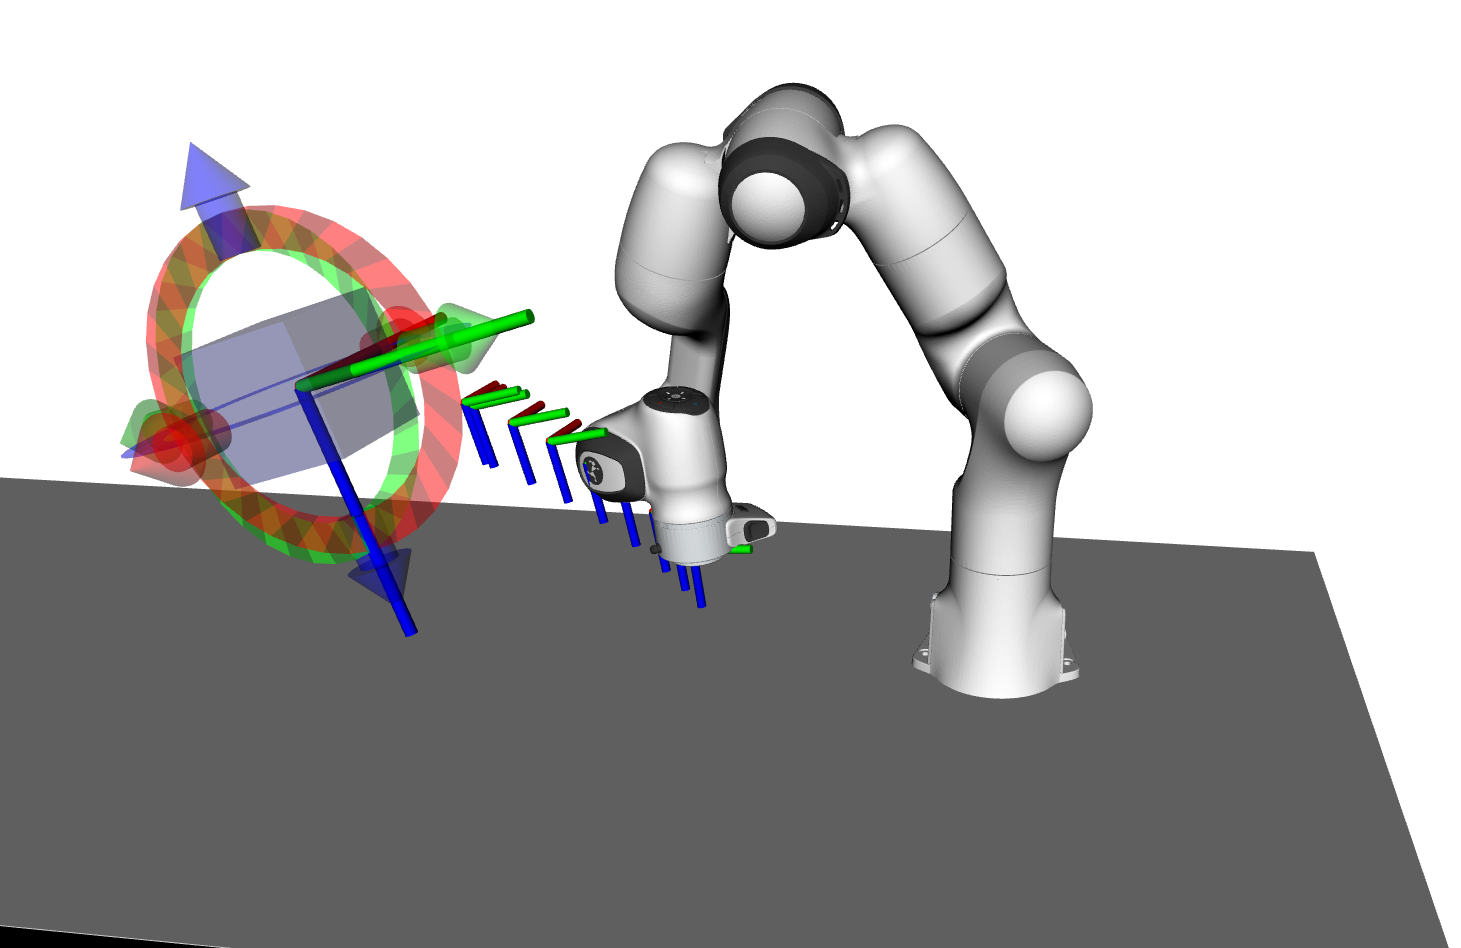
\includegraphics[width=1\linewidth]{Figures/1.png}
\caption{
  \prevrev{fig:example5}
  One final example with a png file.
  }
\label{fig:example5}
\end{figure}
    % INTRO

\include{Chapters/Chapter2}    % LINEAR POSE
% \include{Chapters/Chapter2p} % ark
% \include{Chapters/Chapter2f} % ex fundamentals

\include{Chapters/Chapter3}    % ICRA
% \include{Chapters/Chapter31} % icra

\include{Chapters/Chapter4}    % IROS
% \include{Chapters/Chapter32} % iros

\include{Chapters/Chapter5}    % MPC POLYTOPES
% \include{Chapters/Chapter4p} % journal

\include{Chapters/Chapter6}    % CONCLUSIONS



%----------------------------------------------------------------------------------------
% THESIS CONTENT - APPENDICES
%----------------------------------------------------------------------------------------
\appendix % Cue to tell LaTeX that the following "chapters" are Appendices

% Include the appendices of the thesis as separate files from the Appendices folder
% Uncomment the lines as you write the Appendices
% !TEX root = ../main.tex

%----------------------------------------------------------------------------------------
% APPENDIX TEMPLATE
%----------------------------------------------------------------------------------------

\chapter{Appendix Title Here} % Main appendix title

\label{ApendixX} % Change X to a consecutive letter; for referencing this appendix elsewhere, use \ref{AppendixX}

Write your Appendix content here.

% from https://www.zhaw.ch/en/lsfm/study/studiweb/master-ls/masters-thesis/
% % !TEX root = ../main.tex

\chapter{State-Space Representation}

One of the main interests of the current work is to find a compact
representation of a robot's dynamics that correctly reflects the kinodynamics
constraints in its actuators:

\begin{align}
  \module{\q} & \leq \qub \\
  \module{\qdot} & \leq \qdotub \\
  \module{\tautorque} & \leq \tauub \\
  \module{\tautorquedot} & \leq \taudotub
                           \shortintertext{where} & \nonumber \\
  \tautorque,\tautorquedot &: \text{represent the joint torque and its derivative} \nonumber
\end{align}

Given ${\poselog=[\pos\ \rotlog]^T \in \sethree}$, where ${\pos
  \incoordspace{R}{3}, \rotlog \in\sothree}$, and joint configuration,
velocity and torques: ${\q,\qdot,\tautorque \incoordspace{R}{n}}$ in a n-dof
serial robot, we can use a system state ${\x=[\poselog\ \q\ \qdot\
  \tautorque]^T}$, along with the
joint torque rate as input ${\uinput=\tautorquedot \incoordspace{R}{n}}$, to arrive at a compact
representation of the system:

\begin{gather}
  \xdot = \A \x + \B \uinput + \V \label{eqn:ss_generic} \\
  \label{eqn:ss_continuous}
  \underbrace{\left[
      \begin{array}{c}
        \twist \\
        \qdot \\
        \qddot \\
        \tautorquedot
      \end{array}\right]}_{\xdot}=
  \underbrace{\left[
      \begin{array}{ccccc}
          & 0 & 0 & \jac & 0 \\
         &&& \eye{n} & 0 \\
          &&&& \imat^{-1} \\
          &&&& 0
      \end{array}\right]}_{\A}
  \underbrace{\left[
      \begin{array}{c}
        \poselog \\
        \q \\
        \qdot \\
        \tautorque
      \end{array}\right]}_{\x}
  + \underbrace{
    \left[
      \begin{array}{ccc}
        0 \\
        0 \\
        0 \\
        \eye[ n ]
      \end{array}\right]}_{\B}
  \underbrace{\tautorquedot_{k}}_{\uinput}
  + \underbrace{
    \left[
      \begin{array}{ccc}
        0 \\
        0 \\
        -\imat^{-1}\biasforces \\
        0
      \end{array}\right]}_{\V}
\end{gather}

\section{Acceleration Observers}

\section{Joint Acceleration Observer}

To measure the joint acceleration, we define a discrete state-space observer can
be designed each time-step as:

\begin{gather}
  \y_k = \C_k\x_k + \D_k \uinput_k + \W_k \label{eqn:ss_discrete_observer}
\end{gather}

Using~\labelcref{eqn:dynmodel}, and treating the term $-\imat^{-1}\biasforces$
as noise, we arrive at the observer expression in the form of~\labelcref{eqn:ss_discrete_observer}:

\begin{gather}
  \underbrace{\qddot_k}_{\y_k} = \underbrace{\left[ \begin{array}{cccc} 0&0&0&\imat^{-1}\end{array}\right]}_{\C_k}
  \x_k +
  \underbrace{\left[ \begin{array}{c} 0\end{array}\right]}_{\D_k}
  \uinput_k +
  \underbrace{-\imat^{-1}\biasforces}_{\W_k}
 \label{eqn:ss_joint_acceleration_observer}
\end{gather}



\section{Operational-space Observer}
In order to track the state of the end-effector, a discrete state-space observer
can be designed with the same form as~\labelcref{eqn:ss_discrete_observer}, this time with $\y = [\pos\ \posdot\ \posddot]^T$ representing the end-effector position
and its derivatives.

Assuming the $\jacdot\qdot$ term in $\posddot=\jac \qddot + \jacdot \qdot$ can
be treated as noise, and using~\labelcref{eqn:dynmodel}, we arrive at a matricial formulation:

\begin{gather}
  \label{eqn:ss_ee_observer}
  \underbrace{\left[
      \begin{array}{c}
        \pos_k \\
        \posdot_k \\
        \posddot_k
      \end{array}\right]}_{\y_k}=
  \underbrace{\left[
      \begin{array}{cccc}
        \eye{d} & 0 & 0 & 0 \\
                && \jac & 0  \\
                &&& \jac \imat^{-1}
      \end{array}\right]}_{\C_k}
  \underbrace{\left[
      \begin{array}{c}
        \pos_k\\
        \q_k\\
        \qdot_k\\
        \tautorque_k
      \end{array}\right]}_{\x_k}
  + \underbrace{\left[
      \begin{array}{c}
        0
      \end{array}\right]}_{\D_k}
  \underbrace{\tautorquedot_{k}}_{\uinput_k}
  + \underbrace{\left[
      \begin{array}{c}
        0 \\
        0 \\
        -\jac\imat^{-1}\biasforces + \jacdot \qdot
      \end{array}\right]}_{\W_k}
\end{gather}

\section{Discretizing the Current System}
\label{sec:discretization_lti_current_system}

Given $\A_c$ in~\labelcref{eqn:ss_continuous} is nillpotent from power 3, we can find
exact expressions for $\A_d,\K, \B_d$ by using their taylor series:

\begin{align}
  \A_d &= \underbrace{\eye[ n ]}_{k=0} + \underbrace{\left[
         \begin{array}{cccc}
           0 & 0 & \jac T_s & 0 \\
           0 & 0 & \eye[ n ] T_s & 0 \\
             &&& \imat^{-1} T_s \\
             &&& 0
         \end{array}\right]}_{k=1} + \underbrace{\left[
                 \begin{array}{cccc}
                   0 & 0 & 0 & \jac \imat^{-1} \frac{T_s^2}{2}\\
                   0 & & 0 & \imat^{-1} \frac{T_s^2}{2} \\
                     &&& 0 \\
                     &&& 0
                 \end{array}\right]}_{k=2} \\
  \Rightarrow \A_d &= \left[
                     \begin{array}{cccc}
                       \eye[ n ] & 0 & \jac T_s & \jac \imat^{-1} \frac{T_s^2}{2} \\
                               & \eye[ n ] & \eye[ n ] T_s & \imat^{-1} \frac{T_s^2}{2} \\
                               &&\eye[ n ]& \imat^{-1} T_s \\
                               &&& \eye[ n ]
                     \end{array}\right]
\end{align}

\begin{align}
  \K &= \underbrace{\eye[ n ] T_s}_{k=1, \text{ }\frac{A_c^0 T_s^1}{1}} + \underbrace{\left[
       \begin{array}{cccc}
         0 & 0 & \jac \frac{T_s^2}{2} & 0 \\
         0 & 0 & \eye[ n ] \frac{T_s^2}{2} & 0 \\
           &&& \imat^{-1} \frac{T_s^2}{2} \\
           &&& 0
       \end{array}\right]}_{k=2, \text{ }\frac{A_c T_s^2}{2}} + \underbrace{\left[
               \begin{array}{cccc}
                 0 & 0 & 0 & \jac \imat^{-1} \frac{T_s^3}{6} \\
                   & & 0 & \imat^{-1} \frac{T_s^3}{6} \\
                   &&& 0 \\
                   &&& 0
               \end{array}\right]}_{k=2,\text{ }\frac{A_c^2 T_s^3}{6}} \\
  \Rightarrow \K &= \left[
                   \begin{array}{cccc}
                     \eye[ n ]T_s & 0 & \jac \frac{T_s^2}{2} & \jac \imat^{-1} \frac{T_s^3}{6} \\
                                & \eye[ n ]T_s & \eye[ n ] \frac{T_s^2}{2} & \imat^{-1} \frac{T_s^3}{6} \\
                                &&\eye[ n ]T_s& \imat^{-1} \frac{T_s^2}{2} \\
                                &&& \eye[ n ]T_s
                   \end{array}\right]
\end{align}

With:
\begin{align}
  \Rightarrow \B_d&= \K \B_c \\
                  &= \left[
                    \begin{array}{c}
                      \jac \imat^{-1} \frac{T_s^3}{6} \\
                      \imat^{-1} \frac{T_s^3}{6} \\
                      \imat^{-1} \frac{T_s^2}{2} \\
                      \eye[ n ]T_s
                    \end{array}\right] \\
  \Rightarrow \V_d&= \K \V_c \\
                  &= \left[
                    \begin{array}{c}
                      -\frac{T_s^2}{2} \jac \imat^{-1}\biasforces \\
                      -\frac{T_s^2}{2} \imat^{-1}\biasforces \\
                      -T_s \imat^{-1}\biasforces \\
                      0
                    \end{array}\right] \\
\end{align}


\section{Generalizing Cartesian-space Tracking with Observer in a receding horizon}

Using the end-effector observer (~\labelcref{eqn:ss_ee_observer}) with an adequately
designed weight matrix $\Q$, we
can formulate the MPC tracking strategy as a quadratic problem of minimizing the
squared distance between $\y$ and the references trajectory points $\y^*$ for
the whole horizon (developped in~\Cref{sec:leastsquare_qp}):
\begin{gather}
  \underset{\z}{\text{min }J} = ||\yoover(\z) - \yoover^*||^2_{\Q} \label{eqn:mpc_cost}
\end{gather}
s.t.
\begin{align}
  \xover &= \Ahat \xhat + \Bhat \uinputhat + \Vhat \label{eqn:ss_z_equality} \\
         &= \left[
           \begin{array}{cc}
             \Ahat & \Bhat
           \end{array}\right]
                     \left[\begin{array}{c}
                             \F_{\xhat} \\
                             \F_{\uinputhat}
                           \end{array}\right] \z + \Vhat \\
  \yoover(\z) &= \Coover \xoover + \Doover \uinputoover + \Woover \label{eqn:ss_z_observer} \\
         &= \left[
           \begin{array}{cc}
             \Coover & \Doover
           \end{array}\right]
                     \left[\begin{array}{c}
                             \F_{\xoover} \\
                             \F_{\uinputoover}
                           \end{array}\right] \z + \Woover \\
  \shortintertext{where:}
  \y_k &= [\pos_k,\posdot_k,\posddot_k]^T \\
  \x_k &= [\pos_k,\qdot_k,\qddot_k,\tautorque_k]^T \\
  \xhat &= \F_{\xhat} \z  = [\x_0, \x_1,...,\x_{H-1}]^T \\
  \uinputhat &= \F_{\uinputhat} \z = [\uinput_0, \uinput_1,...,\uinput_{H-1}]^T \\
  \yhat &= [\y_0, \y_1,...,\y_{H-1}]^T \\
  \yhat^*&= [\y_0^*, \y_1^*,...,\y_{H-1}^*]^T \\
  \xover &= \F_{\xover} \z = [\x_1, \x_2,...,\x_H]^T \\
  \yover &= [\y_1, \y_2,...,\y_H]^T \\
  \xoover &= \F_{\xoover} \z = [\x_1, \x_2,...,\x_{H-1}]^T \\
  \uinputoover &= \F_{\uinputoover} \z = [\uinput_1, \uinput_2,...,\uinput_{H-1}]^T \\
  \yoover &= [\y_1, \y_2,...,\y_{H-1}]^T \\
  \Vhat &= [\underbrace{\V_0, \V_0,...,\V_0}_{H}]^T, \What = [\underbrace{\W_0, \W_0,...,\W_0}_{H}]^T
\end{align}

\textbf{About the Equality Constraint}

To clarify~\labelcref{eqn:ss_z_equality}, it's developed below:

\begin{gather}
  \smaller
  \xover = \Ahat \xhat + \Bhat \uinputhat + \Vhat \tag*{~\labelcref{eqn:ss_z_equality}  revisited} \\
  -\Vhat = \Ahat \xhat + \Bhat \uinputhat -\xover \\
  -\Vhat = \left[
    \begin{array}{ccc}
      \Ahat & \Bhat & -\eye[ n_{\xover} ]
    \end{array}\right]
  \left[\begin{array}{c}
          \F_{\xhat} \\
          \F_{\uinputhat} \\
          \F_{\xover}
        \end{array}\right] \z
\end{gather}

\begin{gather}
        -\underbrace{\left[
          \begin{array}{c}
            \V \\
            \V \\
            \vdots \\
            \V
          \end{array}\right]}_{\Vhat} =
      \underbrace{\left[
          \begin{array}{c|c|c}
            \begin{array}{ccccc}
              \A\\
              &\A\\
              &&\ddots\\
              &&&\A
            \end{array}
              & \begin{array}{ccccc}
                  \B\\
                  &\B\\
                  &&\ddots\\
                  &&&\B
                \end{array}
              & \begin{array}{c}
                  -\eye[ n_{\xover} ]
                \end{array}
          \end{array}\right]}_{\left[ \begin{array}{c|c|c} \Ahat & \Bhat & -\eye[ n_{\xover} ] \end{array}\right]}
      \underbrace{\left[
          \begin{array}{ccc}
            \eye[ n_{\xhat}\times n_{\xhat} ]
            & \zeros[ n_{\xhat}\times n_x ]
            & \zeros[ n_{\xhat}\times n_{\uinputhat} ] \\
            \hline
            \zeros[ n_{\uinputhat}\times n_{\xhat} ]
            & \zeros[ n_{\uinputhat}\times n_x ]
            & \eye[ n_{\uinputhat}\times n_{\uinputhat} ] \\
            \hline
            \zeros[ n_{\xover}\times n_x ]
            & \eye[ n_{\xover}\times n_{\xover} ]
            & \zeros[ n_{\xover}\times n_{\uinputhat} ]
          \end{array}\right]}_{\left[\begin{array}{c}
                                       \F_{\xhat} \\
                                       \hline
                                       \F_{\uinputhat}\\
                                       \hline
                                       \F_{\xover}
                                     \end{array}\right]}
      \underbrace{\left[
          \begin{array}{c}
            \x_0 \\
            \x_1 \\
            \x_2 \\
            \vdots \\
            \x_{H-1} \\
            \x_H \\
            \uinputhat
          \end{array}\right]}_{\z} \\
      \shortintertext{with:} \nonumber \\
      n_z = n_x+n_{\xhat}+n_{\uinputhat} \\
      n_{\xhat} = Hn_x \\
      n_{\uinputhat} = Hn_{\uinput}
\end{gather}

\textbf{About the observer Cost Function}

It's important to note in~\labelcref{eqn:ss_ee_observer}, $\D=0$ (and thus in $\Doover$ in~\labelcref{eqn:ss_z_observer}),  to make it more clear:

\begin{gather}
  \yoover(\z) = \Coover \xoover + \Doover \uinputoover + \Woover \tag*{~\labelcref{eqn:ss_z_observer}  revisited} \\
  \yoover(\z) = \Coover \underbrace{\F_{\xoover} \z}_{\xoover} + \Woover \\
  \smaller
  \underbrace{\left[
      \begin{array}{c}
        \y_1 \\
        \y_2 \\
        \y_3 \\
        \vdots \\
        \x_{H-1}
      \end{array}\right]}_{\yoover}=
  \underbrace{\left[
      \begin{array}{ccccc}
        \C \\
        & \C \\
        & & \C \\
        &&&\ddots \\
        & & & & \C \\
      \end{array}\right]}_{\Coover}
  \underbrace{\left[
      \begin{array}{ccccc}
        \zeros[ n_{\xoover}\times n_x ]
        & \eye[ n_{\xoover}\times n_{\xoover} ]
        & \eye[ n_{\xoover}\times n_x ]
        & \zeros[ n_{\xoover}\times n_{\uinput} ]
        & \zeros[ n_{\xoover}\times n_{\uinputoover} ]
      \end{array}\right]}_{\F_{\xoover}}
  \underbrace{\left[
      \begin{array}{c}
        \x_0 \\
        \xoover \\
        \x_H \\
        \uinput_0 \\
        \uinputoover
      \end{array}\right]}_{\z}
  +
  \underbrace{\left[
      \begin{array}{c}
        \W \\
        \W \\
        \vdots \\
        \W
      \end{array}\right]}_{\Woover} \\
  \shortintertext{with:} \nonumber \\
  n_z = n_x+n_{\xoover}+n_x+n_{\uinputhat} \\
  n_{\uinputhat} = n_{\uinputoover} + n_{\uinput} \\
  n_{\uinputoover} = (H-1)n_{\uinput} \\
  n_{\xoover} = (H-1)n_x
\end{gather}


\section{Using the generalized observer for position tracking}
For an adequately chosen $\Q$, we can extract the end-effector pose and
define que the cost function~\labelcref{eqn:mpc_cost} in such a way that:

\begin{gather}
  \underset{\z}{\text{min }J} = ||\posoover(\z) - \posoover^*||^2_{\Q} \label{eqn:mpc_pos_cost}
\end{gather}

where $\posoover = [\pos_1,\pos_2, ..., \pos_{H-1}]^T$, and likewise for the
reference trajectory in the horizon~$\posoover^*$.

As for $\Q$, it's defined in such a way that:
\begin{gather}
  (\yoover - \yoover^*)^T\Q(\yoover - \yoover^*) =
  (\posoover - \posoover^*)^T\Q(\posoover - \posoover^*) \\
  \Q = \left[
    \begin{array}{ccccc}
      \F_{\pos} \\
      & \F_{\pos} \\
      & & \F_{\pos} \\
      &&&\ddots \\
      & & & & \F_{\pos} \\
    \end{array}\right] \\
\shortintertext{with:} \nonumber\\
\pos_k = \F_{\pos} \y_k \\
\F_{\pos}=
\left[
  \begin{array}{ccc}
    \eye[ n_d\times n_d ] \\
    & \zeros[ n_d\times n_d ] \\
    & & \zeros[ n_d\times n_d ]
  \end{array}\right]
\end{gather}

Where $n_d$ is the dimension of the workspace.

%\include{Appendices/AppendixC}
% % !TEX root = ../main.tex

%----------------------------------------------------------------------------------------
% APPENDIX: DECLARATION OF ORIGINALITY
%----------------------------------------------------------------------------------------

% Include the official "Plagiatserklärung" as a PDF

% Ensure that a TOC entry is create while suppressing the chapter header
\cleardoublepage
\phantomsection
\addtocounter{chapter}{1}
\addcontentsline{toc}{chapter}{\protect\numberline{\thechapter} Declaration of Originality}
% The above replaces this command (which creates a chapter header).
%\chapter{Declaration of Originality} % Main appendix title
\label{DeclarationOfOriginalityZHAW}

% Include a PDF (full page)
\includepdf[pages=-]{Appendices/plagiatserklaerung-master-eng.pdf}



%----------------------------------------------------------------------------------------
% BIBLIOGRAPHY
%----------------------------------------------------------------------------------------
\printbibliography[heading=bibintoc]

%----------------------------------------------------------------------------------------

\end{document}
